%\documentclass[11pt,oneside,a4paper]{mr}%one-page printing
\documentclass[11pt,twoside,a4paper]{dp_format}%two-page printing
\usepackage[utf8]{inputenc}
\usepackage[czech]{babel}
\RequirePackage[T1]{fontenc}
%\usepackage[latin2]{inputenc}
\usepackage{graphicx}
\input dp_macro.tex   % specialni makra pro formatovani diplomek

\newcommand\DiplTitle{Systém automatického záznamu televizních pořadů - DVBgrab}
\newcommand\FirstandFamilyName{Martin Jansa}
\newcommand\Month{březen}
\newcommand\Year{2006}
\newcommand\Supervisor{Ing. Ivan Halaška}

\newcommand\StudProgram{Informatika a výpočetní technika}
\newcommand\Faculty{Fakulta elektrotechnická}
\newcommand\University{České vysoké učení technické v Praze}

\begin{document}
\coverpagestarts
\vspace*{\fill}

\cleardoublepage %\thispagestyle{empty}
%*************************************************************************

\vspace*{\fill}
\chapter*{Poděkování}
Děkuji tvůrcům původního projektu TVgrab a obecně všem vývojářům svobodného software, díky kterým tento projekt mohl vůbec vzniknout.

Dále děkuji Kataríně Hanuliakové za pomoc s grafickou úpravou aplikace a slovenský překlad, Zuzaně Moravcové za překlad do francouzštiny a Ivě Höflerové za jazykovou korekturu tohoto textu.

\cleardoublepage %\thispagestyle{empty}
%*************************************************************************

\vspace*{\fill}
\chapter*{Prohlášení}
Prohlašuji, že jsem svou diplomovou práci vypracoval samostatně a použil jsem pouze podklady uvedené v přiloženém seznamu.

Nemám závažný důvod proti užití tohoto školního díla ve smyslu \S 60 Zákona č. 121/2000 Sb., o právu autorském, o právech souvisejících s právem autorským a o změně některých zákonů (autorský zákon).

V Praze 6 dne 29. 3. 2006  \hfill \hbox to 70mm{\tiny\dotfill}
 
\cleardoublepage%\thispagestyle{empty}
%*************************************************************************

\chapter*{Abstract}
The system is intended for easy recording of television shows. Data are taken from local network stream (ie. DVB-T from VideoLanServer). User has to register on the web interface and after login he can see television schedule for next week. Every program is shown as hypertext link and after the confirmation the request for program is saved in a database. There is a neverending loop on the server backend which is searching requests in a database and if any requested program starts, it runs dumping packets from data stream to disk. After finishing it sends an email with hypertext link to requesting users.
\vglue60mm
\chapter*{Abstrakt}
Systém byl vytvořen za účelem usnadnění záznamu televizních pořadů, které jsou vysílány po lokální síti (například pomocí VideoLanServeru z DVB-T vysílání). Uživatel se zaregistruje na webovém rozhraní a po přihlášení si zobrazí televizní program na přibližně týden dopředu. Vybráním pořadu se jeho objednávka zaznamená v databázi. Na serveru běží nekonečná smyčka, která sleduje, zda v databázi není požadavek na pořad, který právě začíná. Při nálezu začne ukládat data z vysílání a po dokončení pošle odkaz na stažení všem uživatelům, kteří daný pořad požadovali.
\cleardoublepage%\thispagestyle{empty}
%*************************************************************************

\tableofcontents
\cleardoublepage%\thispagestyle{empty}
%*************************************************************************

\listoffigures
\addcontentsline{toc}{chapter}{\protect\numberline{}{Seznam obrázků}}
\cleardoublepage%\thispagestyle{empty}
%*************************************************************************

\listoftables
\addcontentsline{toc}{chapter}{\protect\numberline{}{Seznam tabulek}}
\cleardoublepage%\thispagestyle{empty}
%*************************************************************************

\mainbodystarts
\chapter{Co od systému očekáváme}

\section{Z pohledu uživatele}
Uživatel není nucen instalovat žádné dodatečné programy, pouze internetovým prohlížečem přistoupí na stránky aplikace a zadá o jaké pořady má zájem. Před prvním použitím se uživatel na stránkách zaregistruje, čímž je automaticky i přihlásen do systému. Stránky komunikují s uživatelem pokud možno jeho preferovaným jazykem podle nastavení prohlížece, případně může zvolit jiny z nabízených. Zvolený jazyk se pamatuje dlouhodobě. Uživatelské jméno a heslo také, takže při dalších návštěvách ze stejného počítače, už není nutné zadávat. Výběr pořadů by měl být minimálně na týden dopředu.

\vspace{10pt}

V seznamu pořadů stačí kliknout na název pořadu a tím je požadavek zadán. Nahraný pořad se po uložení ještě komprimuje do uživatelem zvoleného formátu.

\vspace{10pt}

Po uložení a zkomprimování je do uživatelova adresáře uložen odkaz na pořad a o jeho připravenosti je uživatel informován emailem. Odkaz může být bud přes protokol ftp nebo http. O hotových nahrávkách se může také informovat v rámci webového rozhraní, kde je seznam jeho nahrávek včetně odkazů na stažení, objednaných nahrávek a hotových nahrávek všech uživatelů.

\vspace{10pt}

Uživatel má možnost měnit některé parametry svého účtu, nechat si zaslat nově vygenerované heslo a úplně zrušit účet.

\vspace{10pt}

\section{Z pohledu správce}
Potřebujeme přehlednou a automatickou správu uživatelů, Potřebujeme aby systém korektně reagoval na výpadky spojení s databází nebo na nedostatek diskového prostoru.

Pro možnosti použití i mimo Ceskou Republiku je třeba použít ve webovém rozhraní kódování podporující více národních abeced (UTF-8) a podle toho také zajistit správné kódování znaků u dat přicházejících z databáze přes ADOdb. Také televizní program se nutné načítat v nějakém srozumitelném, dobře definovaném a mezinárodně uznávaném formátu jako je XMLTV viz. \cite{xmltvURL}. To značně usnadňuje instalaci v zahraničí, kde je obvykle dostatek zdrojů programu v XMLTV. Přidávání nových kanálů musí být co nejsnažší a nesmí vyžadovat hlubší znalosti systému.

\vspace{10pt}

\chapter{Popis systému}

Systém je založen na starším projektu TVgrab, který implementoval nahrávání z klasického analogového signálu a jedinou podporovanou databází byla MySQL. Tento systém byl upraven pro nahrávání z libovolného zdroje šířeného v lokální síti a veškeré databázové funkce jsou nyní volány přes ADOdb. Další provedené změny viz. soubor changelog.

\vspace{10pt}

\section{Servery}
Systém využívá ke svému běhu 2 různé servery, i když to není nutností. Na jednom běží databáze a webové rozhraní. Na druhém potom vysílání signálu do lokální sítě, záznam na disk a distribuce nahraných pořadů.

\vspace{10pt}

\section{Databáze}

\vspace{10pt}

Jako databázový server lze použít téměř libovolnou SQL databázi, protože systém využívá knihovny ADOdb, která podporuje v současné době zhruba 15 různých databázových strojů. Systém byl provozován na MySQL databázi, nyní na PostgreSQL. Kvůli použití ADOdb je nutné vždy volat SQL kód jen s použitím ADOdb funkcí, třeba pro formátování datumu v SQL dotazech musí být vždy volána odpovídající ADOdb funkce, která vygeneruje funkci odpovídající aktuálně použitému databázovému serveru.

\vspace{10pt}

\section{Webové stránky}

\vspace{10pt}

Webové prostředí je napsáno pomocí XHTML+PHP+JavaScript. Obsahuje jak uživatelské tak administrativní rozhraní převážně pro prvotní nastavení a případné změny v konfiguraci. Je napsáno s podporou více jazykových variant (čeština, slovenština, angličtina, francouzština). Všechny zobrazované texty jsou definovány jako konstanty v souborech lang/lang.jazyk.php.

\vspace{10pt}

Jazyk se volí postupně podle těchto pravidel: 

\vspace{10pt}

1) podle cookie, pokud uživatel někdy přepnul jazyk ručně kliknutím na ikonu vlajky

2) podle preferovaných jazyků v nastavení prohlížeče

3) v databázi hledáme poslední použitý jazyk daného uživatele

4) výchozí jazyk definovaný v globální konfiguraci

\vspace{10pt}

Nakonec se zvolený jazyk uloží do databáze k uživateli jako poslední použitý jazyk. To se využívá například při odesílání e-mailu o úspěšném nahrání, kdy nemáme k dispozici uživatele, jeho cookies ani jeho prohlížeč.

\vspace{10pt}

Z důvodu vícejazyčného webového rozhraní je třeba zajistit také kódování v databázi nastavené na UTF-8, aby podporovala všechny přípustné varianty.

\vspace{10pt}

\section{Záznam}

\vspace{10pt}

O nahrávání se starají 2 nekonečné smyčky naprogramované také v PHP, jedna se stará o záznam (grab\_loop), druhá o komprimaci (encode\_loop). Záznamová smyčka se nastartuje po startu systému a po krátkych časových intervalech kontroluje, zda na některém kanálu nezačíná nějaký objednaný pořad. 
Pokud ano, spustí na pozadí nový proces, který zajistí záznam tohoto pořadu (grab\_process, kterému se předává pouze ID záznamu v databázi) a sama pokračuje dál ve své činnosti.

Komprimační smyčka je odlišná, startuje se sice také po startu systému, ale protože nemá smysl pouštět paralelně příliš mnoho komprimačních procesů, tak vždy kontroluje, zda existuje v databázi nějaký nevyřízený požadavek na formát, do kterého se zrovna nic nekomprimuje. Pokud ano, vybere nejstarší podle data vysílání pořadu a spustí nový proces (encode\_process, kterému předává ID požadavku a formát, jaký se má použít). To znamená, že kolik různých formátů si uložíme do databázové tabulky encoder, tolik komprimačních procesů může běžet paralelně.

\vspace{10pt}

Vlastní záznam na disk je prováděn pomocí programu dumprtp, z balíku dvbstream, který ukládá datový tok ze zadané IP adresy a portu do souboru. V záznamovém procesu se nejdříve všechny požadavky na daný pořad přepnou ze stavu "naplánován" do stavu "ukládá se". Poté je dumprtp spouštěn jako volání podprocesu na pozadí a poté je počítán čas až do konce pořadu, kdy se pošle procesu dumprtp signál TERM k ukončení. 

\vspace{10pt}

Data se při ukládání netransformují, takže zůstanou uložena jako MPEG-TS (transport stream). To umožňuje paralelní zápis několika pořadů na disk, protože je to operace relativně nenáročná. Transport stream je optimalizovaný spíše pro přenos audio video signálů, než pro jejich přehrávání (neobsahuje příliš často klíčové snímky, takže například při posunech je dlouhá odezva než se obnoví obraz). Z jaké IP adresy a portu se má ukládat, je nyní určeno v databázi v definici televizního kanálu.

\vspace{10pt}

Jmenné konvence pro název nahrávky jsou DVB- jako předpona, pak datum ve formátu Ymd-Hi (rok, měsíc, den, hodiny, minuty) tak, aby se adresář s nahrávkami dal řadit chronologicky podle abecedy, dále následuje jméno kanálu (po odstranění diakritiky) a název pořadu, buď po odstranění diakritiky nebo jenom ID záznamu, pokud to je v konfiguraci nastaveno (přesné jméno pořadu včetně diakritiky je pak až v popisném XML souboru viz dále. Nekomprimované nahrávky mají příponu .ts jako transport stream.

\vspace{10pt}

Po ukončení dumprtp se ještě zkontroluje, zda má nahrávka nějakou rozumnou nenulovou velikost a informace o uložení se aktualizuje v databázi (všechny požadavky na tento pořad přejdou ze stavu "ukládá se" do stavu "uložen".

\vspace{10pt}

\section{Specifika ukládání z DVB vysílání}

\vspace{10pt}

Součástí DVB vysílání jsou i informace o vysílaných pořadech.

Tyto informace jsou vysílány jako součást MPEG-2 dat pomocí protokolu PMCP (Programming Metadata Communication Protocol), což jsou do XML balené data z PSIP (Program and System Information Protocol).

\vspace{10pt}

Součástí PSIP jsou následující tabulky:

* STT (system time table) - aktuální čas vysílaný každou sekundu

* MGT (master guide table) - datové ukazatale do dalších tabulek PSIP

* VCT (virtual channel table) - seznam kanálů a přiřazení jejich čísel

* RRT (rating region table) - hodnocení obsahu pro jednotlivé regiony

* EIT (event information table) - názvy a další data pro televizní program

* ETT (extended text table) - detailní popis programů

* DCCT (directed channel change table)

* DCCST (directed channel change selection code table)

\vspace{10pt}

Tabulky EIT a ETT používá v MHP (Multimedia Home Platform - aplikační rozšíření v DVB) aplikace EPG (Electronic program guide - elektronický televizní program). Tyto informace by bylo velmi výhodné použít pro přesné nastavení začátku a konce záznamu.

\vspace{10pt}

Pokud toto nemáme k dispozici, musí nahrávání začínat několik minut před plánovaným začátkem pořadu (lze konfigurovat kolik) a také lze nastavit kolik minut se má nahrávat po plánovaném konci pořadu.

\vspace{10pt}

Pokud bychom chtěli využít informace z EIT přímo v DVBgrabu, tak bychom museli nejdříve zajistit jejich distribuci z vysílajícího serveru do lokální sítě.

\vspace{10pt}

Podle zástupců Czech Digital Group jsou prý tyto údaje již dostupné. Pokud jim televize údaje dodá, tak je pouze převedou do formátu vhodného pro EIT a vloží do toku dat.

\vspace{10pt}

Pokud by v EIT byly obsaženy i značky začátku a konce televizní reklamy, tak by šlo podle nich vypínat a zapínat záznam a tím zajistit automatické vystřihování reklamy. Případně by bylo možné naprogramovat nějaký vlastní algoritmus pro poznávání reklamy (třeba podle podobnosti s dodanou počáteční a koncovou znělkou). Tento algoritmus by byl pravděpodobně dosti hardwarově náročný, což by při několika paralelních záznamech mohlo vést až ke ztrátám snímku, proto nebyl použit. Také tyto algoritmy nemusí být v souladu se zákonem (automatický systém na vystřihování reklamy byl součástí software DVD rekordérů KISS a musel být odstraněn a zůstalo pouze automatické přetáčení reklamy při sledování ze záznamu).

\section{Komprimace záznamů}

Komprimační smyčka postupně prochází přes všechny formáty (encodery) a zkoumá, zda pro ty, které aktuálně neběží (nemají v databázi uložené své číslo procesu PID), neexistuje nějaký čekající požadavek ve stavu "uložen". Pokud ano, vybere opět nejstarší. Založí na pozadí nový proces, který komprimaci zajistí. Komprimační proces nejdříve opět změní stav požadavku v databázi z "uložen" na "komprimuje se". 
Poté spustí skript, jehož jméno je opět uvedeno v databázi a který musí být uložen v adresáři encoders, tomuto skriptu předá název nahraného pořadu, který do databáze uložil předcházející záznamový proces a z původního jména vytvoří název cílového souboru připojením definované přípony z databáze. Po úspěšné komprimaci je z .ts souboru vytvořen například .avi soubor ve formátu MPEG-4, znovu se zkontroluje, zda výsledný soubor má rozumnou velikost a pokud ano, dojde k uveřejnění nahrávky požadujícím uživatelům. 

\vspace{10pt}

\section{Komprimační formáty}

Komprimaci zajišťuje program mencoder, který podporuje velmi mnoho formátů. Některé základní jsem uvedl v příloze.
Protože nemá smysl umožňovat uživateli komprimovat nahrávky do libovolné přípustné kombinace kontejner, video, audio kodek. 

\vspace{10pt}

Tak je připraveno pouze pár zajímavých kombinací a to:

\vspace{10pt}

MPEG-2 TS - formát v jakém přijímáme DVB signál ze sítě, soubor bude mít příponu .mpg.

AVI/MPEG-4 ASP (z libavcodec)/MP3 - běžně používaný komprimovaný soubor, hodina záznamu odpovídá zhruba 700MB. Předdefinované varianty s různým měřítkem (různé rozlišení), soubor bude mít příponu .avi.

\vspace{10pt}

Dále by bylo vhodné použít:

\vspace{10pt}

OGG/Theora/Vorbis - svobodná obdoba předchozí kombinace s trošku efektivnějším poměrem kvality a velikosti souboru, s příponou .ogg.

MP4/MPEG-4 AVC (z x264)/AAC - nejvyšší kvalita, pokud budeme mít dostatečně kvalitní zdroj, přípona by byla .mp4.

\vspace{10pt}

\section{Uveřejnění nahrávky}

\vspace{10pt}

\textbf{Popisný XML soubor}

Vytvoření XML souboru popisujícího detaily nahrávky. Obsahující název pořadu s diakritikou, název kanálu s diakritikou, začátek a konec pořadu podle televizního programu, začátek a konec nahrávání, použitý komprimační formát, výsledná velikost souboru v kB a MD5 součet pro kontrolu bezchybného stažení.

XML soubor je ve webovém prohlížeči zobrazován v podobě přehledné tabulky, která je z XML souboru vytvořena podle XSL šablony.

Ta je v uživatelském adresáři vygenerována (podle jazyku, který uživatel používá na webovém rozhraní DVBgrabu) v souboru dvbgrab.xsl. Pokud uživatel chce stejně zobrazovat i stažené XML soubory, musí k nim do adresáře zkopírovat i tento soubor.

\vspace{10pt}

\textbf{Kontrola a případné založení uživatelského adresáře}

Během vytváření symbolických odkazů dojde také ke kontrole, zda je uživatelský adresář již založen a případně také k přegenerování souboru .htaccess, který určuje, ze kterých IP adres smí uživatel své nahrávky stahovat (tato IP adresa je vždy pouze jedna a je uložena v databázi u informací o uživateli). Uživatel má možnost přes webové rozhraní zadat její změnu, proto musí docházet k přegenerování těchto .htaccess souborů. Druhá varianta je přegenerování souboru pouze pokud nějaká změna skutečně nastala, to rozhoduje údržbový skript pouštěný pomocí plánovače cron. 

\vspace{10pt}

Oba přístupy mají nějaké výhody, ale i nevýhody. První je nevýhodný například pro uživatele, který při pokusu o stažení nahrávky zjistí, že má zaregistrovanou neaktuální IP a další nahrávku zatím neplánuje. Druhý naopak nepotěší uživatele, který ráno zadá změnu IP, v poledne se mu uloží nahrávka a až do půlnoci nejde stáhnout, když se údržbové skripty budou pouštět jen 1x denně o půlnoci. Řešením je buď dostatečně časté pouštění údržby nebo kombinace obou přístupů. Výchozí nastavení generuje .htaccess soubory v obou případech.

\vspace{10pt}

\textbf{Vytvoření symbolického odkazu}

Vytvoření symbolického odkazu z uživatelova adresáře do sdíleného prostoru, ve kterém jsou uložené všechny nahrávky (jak na nahrávku, tak na odpovídající XML soubor).

\vspace{10pt}

\textbf{Odeslání e-mailu a označení v databázi}

Odeslání informačního e-mailu všem uživatelům, kteří tuto nahrávku v tomto formátu požadovali. A u všech uživatelských požadavků je v databázi nastaveno jméno souboru s nahrávkou, jak bude přístupná přes http server, to je pak použito pro generování odkazů na stažení v sekci "moje graby".

\vspace{10pt}

\section{Distribuce záznamů}

\vspace{10pt}

Distribuce nahrávek mezi uživatele je zajištěna přes http server apache (nyní ve verzi 2.2.x, která již nemá problémy se soubory většími než 2GB). Alternativně lze použít i nějaký ftp server, který umí autentifikovat uživatele nejlépe proti použité databázi. Pokud potřebujeme generovat uživatelské účty pro ftp server, máme k dispozici pouze uživatelská jména a md5 součty jejich hesel (musíme číst i md5 hesel z externí autorizační databáze).

\vspace{10pt}

\section{Získávání aktuálního televizního programu pro web}

\vspace{10pt}

Stahování aktuálního TV programu je zajištěno přes různé moduly. V adresáři tvgrabbers jsou jednotlivé php skripty. V distribuci je skript tv\_grab\_novinky\_cz/tv\_grab\_novinky\_cz.php, který načítá data ze serveru novinky.cz, stažený html kód je zpracován pomocí regulárních výrazů a jednotlivé pořady jsou uloženy do databáze. Tento skript umí pouze několik programů (čt1, čt2, nova, prima), pro načítání jiných je nutné skript editovat.

\vspace{10pt}

XMLTV - dalším skriptem v distribuci je xmltv\_to\_db.php, který lze použít pro vkládání XML souboru ve formátu XMLTV do databázové tabulky television. Nejdříve popíšu, co je to XMLTV. XMLTV je specifikace, jak zapisovat televizní program do XML souborů. Tuto specifikaci využívá velmi mnoho programů viz. \cite{xmltvURL}. Na stránkách XMLTV lze stáhnout též instalační balík, který obsahuje stahovací skripty pro poměrně mnoho zemí. Bohužel není obsažen skript po Českou republiku z důvodu, který uvedu v následující sekci.

\vspace{10pt}

Každý stahovací skript musí být před prvním použítím nakonfigurován (např. tv\_grab\_cz --conf pro skript tv\_grab\_cz). Konfigurace se obvykle skládá z několika obecných dotazů. Dále se vypisuje seznam televizních kanálů, které umí stahovat a pro každý kanál uživatel volí, zda se má stahovat či ne. Poté stačí spustit skript s parametrem udávajícím, na kolik dnů dopředu má stahovat, případně od kolikáteho dne začít (např. tv\_grab\_cz --days 10, stáhne na 10 dní dopředu pro všechny povolené kanály jejich program). Výstupem skriptu je správně formátovaný soubor XML, který ještě potřebujeme transformovat do databáze.

\vspace{10pt}

Protože se nám hodí i koncové časy pořadů, pomůže nám pomocný skript z balíku XMLTV tv\_sort, ten nejen chronologicky seřadí pořady v rámci kanálu, ale také každý pořad doplní koncovým časem (podle počátečního času chronologicky následujícího pořadu). Bohužel tohle selhává u posledních pořadů v rámci dne, kdy následujícím pořadem je až první ranní pořad dalšího dne. Tyto situace se snaží detekovat systém až při vytváření požadavku na nahrání a pokud pořad začíná mezi 1. a 5. hodinou ranní a trvá déle než 4 hodiny, tak se koncový čas nastaví jen na čas počáteční + definovaná konstanta (výchozí hodnota je +2 hodiny). Pokud koncové časy nemáme v databázi vůbec (např. po použití modulu tv\_grab\_novinky\_cz.php, tak se koncový čas určuje také při vytváření požadavku na nahrání.

\vspace{10pt}

Takto předzpracovaný program již můžeme zpracovávat pomocí skriptu xmltv\_to\_db.php. Ten složí pro každý element <programme> 2 SELECT dotazy, INSERT pro vložení a UPDATE pro aktualizaci. První dotaz zjistí, zda v danou dobu na daném kanálu již existuje v databázi pořad se stejným jménem, pokud ano, element je ignorován. Jinak se provede druhý dotaz, který zjišťuje, zda neexistuje v tu dobu pořad s jiným jménem, pokud ano, použije se vygenerovaný UPDATE, pokud ne, použije se INSERT. Pokud se ve vstupním souboru objeví například pořad na kanálu, jehož xmltv id nemáme v databázi DVBgrabu registrováno, vypíše se varování a pořad se také nevkládá.

\vspace{10pt}

\section{Právní aspekty získávání televizního programu z veřejně dostupných webových stránek}

\vspace{10pt}

V zahraničí je běžné, že dostupnost XMLTV formátu programu je částečně podporovaná i státem. 

\vspace{10pt}

U nás tomu bohužel tak není a kvůli tomu v XMLTV distribuci stahovací skript pro Českou republiku v dohledné době asi nenajdeme. Dokonce tam jistou dobu byl již i obsažen. Bohužel firma provozující servery, které sloužili jako zdroj programu pro jinou firmu, která zajišťovala transformaci z HTML formátu do XMLTV, nebyla této aktivitě příznivě nakloněna a tak byl projekt českého XMLTV pod hrozbou žaloby zastaven.

\vspace{10pt}

Bohužel i mě jako tvůrci DVBgrabu byla zaslána žádost o urychlené odstranění načítání televizního programu ze stránek http://www.ceskenoviny.cz, jejichž provozovatelem je Česká tisková kancelář (ČTK), jinak by záležitost řešilo právní oddělení ČTK. Proto nová verze DVBgrabu nebude distribuována včetně českého XMLTV modulu a správce systému je pak nucen použít skript tv\_grab\_novinky\_cz.php (za předpokladu, že snad přátelštější provozovatel http://www.seznam.cz nepřijde s žádostí o odstranění) a nebo si zajistit xmltv zdroj svépomocí.

\vspace{10pt}

Doufejme, že co nejdříve si některý portál nabízející online tv program v HTML podobě všimne na trhu tohoto nedostatku a doplní své portfolio služeb například o placený přístup k XMLTV formátu jejich programu.


\chapter{Vysílání po počítačové síti}

Seznam produktů, které jsou potřeba pro zprovoznění systému a návod k jejich nastavení pro DVBgrab.

\vspace{10pt}

Pro vysílání po sítí se používají programy z projektu VideoLAN \cite{videolanURL}. Jejich použití je následující:

\vspace{10pt}

\begin{figure}[h]
\begin{center}
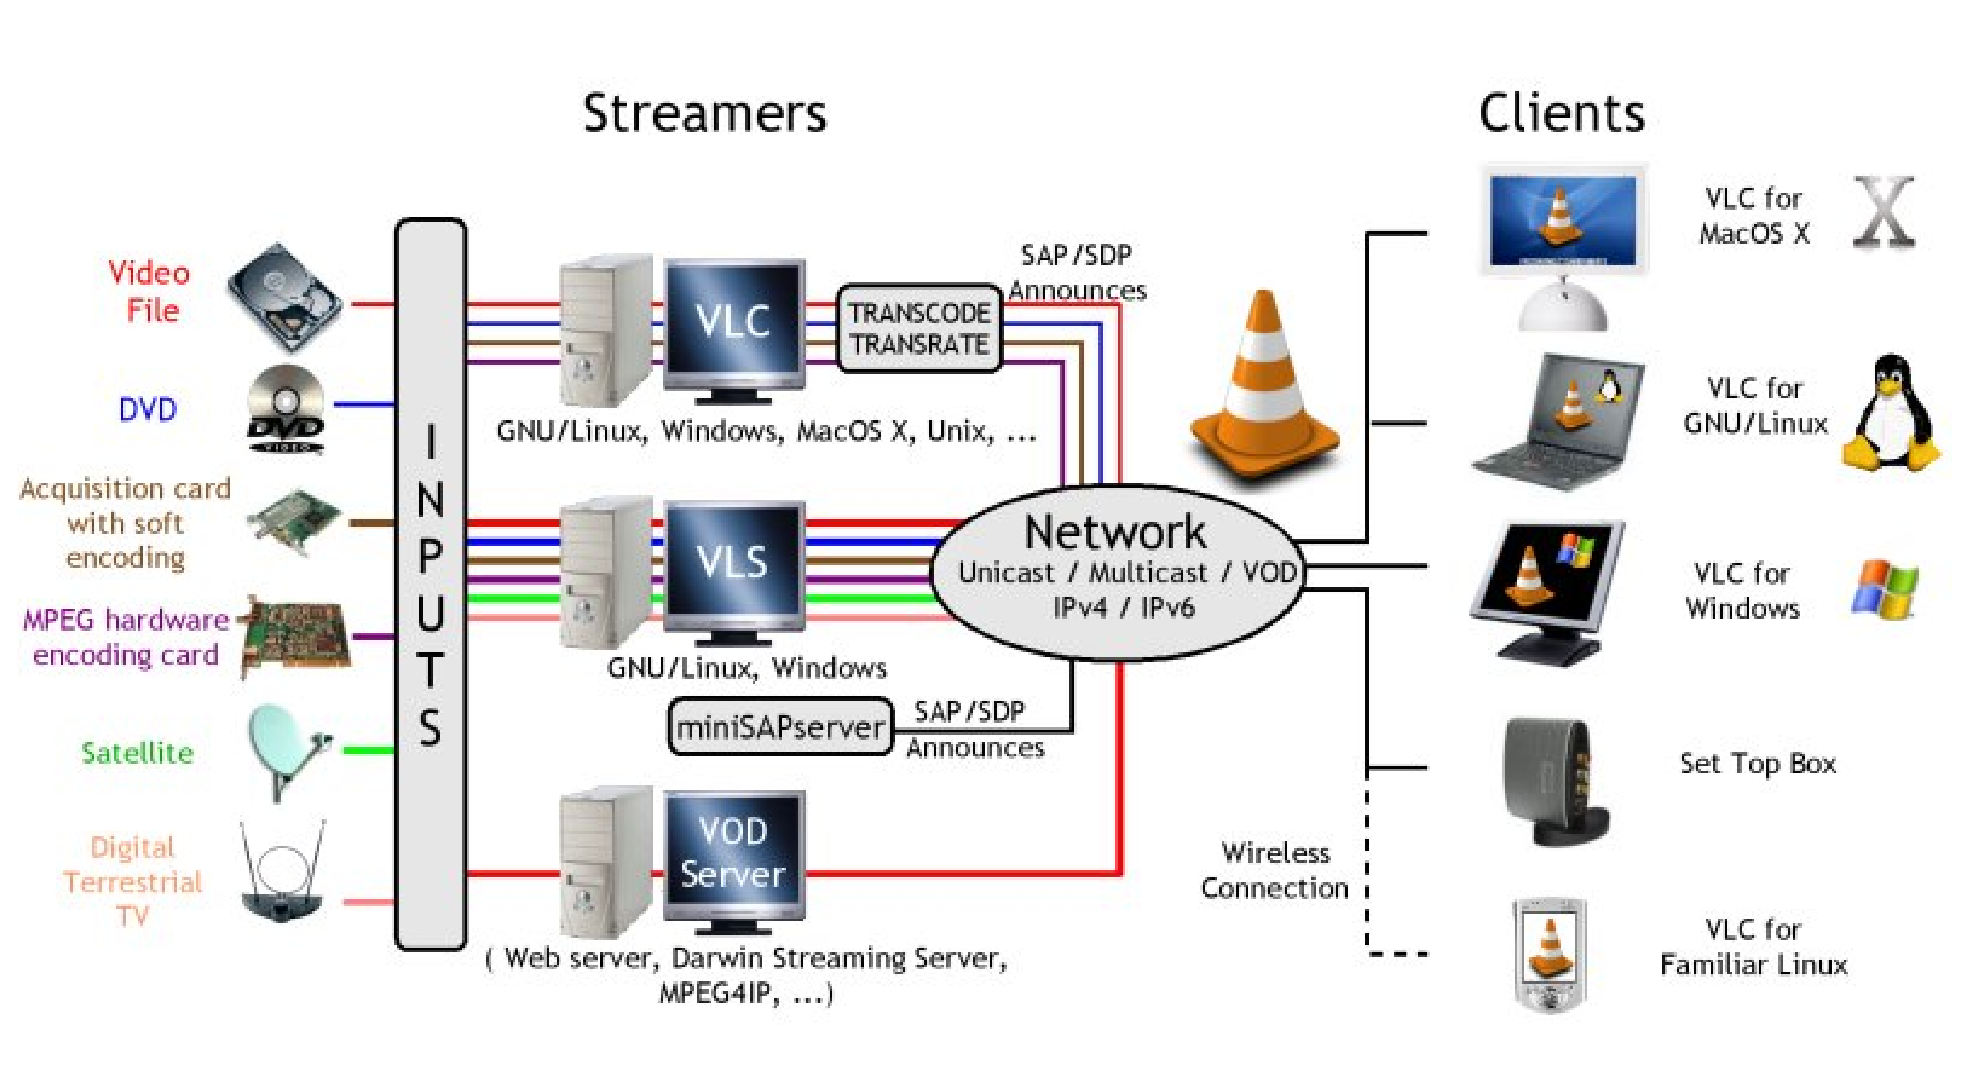
\includegraphics[width=15cm]{images/videolan.eps}
\caption{Využití programů z projektu VideoLAN}
\label{fig:videolan}
\end{center}
\end{figure}

\vspace{10pt}

\section{Příprava na vysílání po síti}


\vspace{10pt}

Pro provozování DVBgrabu je důležitá pouze konfigurace vysílání DVB-T signálů pomocí multicastu. Multicast je totiž nejefektivnější a díky tomu vlastně jediný použitelný pro větší lokální sítě. Konfiguraci a získání seznamu pořadů v multiplexu popíšu v této sekci, přesto pak místo VideoLanServer(VLS)+miniSAPserver může být snazší a rychlejší použít přímo VideoLanClient(VLC) i pro vysílání.

\vspace{10pt}

Nejdříve budeme potřebovat nějaké DVB-T karty, obvykle do slotu PCI. Odzkoušené a ověřené jsou například karty Hauppauge WinTV-NOVA-T (Technotrend Systemtechnik GmbH Technotrend-Budget, Philips Semiconductors SAA7146 rev 01). Pokud chceme paralelně vysílat kanály z více různých multiplexu, potřebujeme více těchto karet. Multiplex v DVB je balík televizních, rozhlasových a datových kanálů, který je vysílán v rámci jedné frekvence po celém území. Každá DVB-T karta má potom na svém tuneru naladěnu frekvenci multiplexu a paralelně přijímá všechny kanály tohoto multiplexu.

\vspace{10pt}

V České Republice jsou v současné době k dispozici 3 DVB-T multiplexy Czech Digital Group (CDG), České Radiokomunikace (CRA), Český Telecom (CTc). CRA nyní vysílá pořady České Televize, CDG má navíc k dispozici televizi Nova, Prima, Očko, 24CZ apod., CTc mají Českou Televizi, Očko, Novu.

\vspace{10pt}

Ovladače těchto karet jsou k dispozici na stránkách projektu linuxtv \cite{linuxtvURL} a také jsou součástí jádra systému řady 2.6. V novějších jádrech než je 2.6.9 se promítlo mnoho změn v ovladačích, proto je potřeba stáhnout i novější verze firmware karty, která se nahrává při načítání ovladače.

\vspace{10pt}

Pro zprovoznění vysílání je vhodné nainstalovat ještě několik uživatelských aplikací jako media-tv/linuxtv-dvb,linuxtv-dvb-apps,linuxtv-dvb-headers,libdvbpsi,dvbsnoop pro Gentoo a dvb-utils,dvbsnoop,dvbstream,dvbtune,libdvb-dev,libdvbpsi3,libdvbpsi3-dev pro debian.

\vspace{10pt}

Pro zjištění dostupných kanálů lze použít například příkaz scan z balíku dvb-utils. Nejdříve je třeba připravit soubor s výchozím nastavením tuneru, aby karta věděla, ve kterém multiplexu chceme kanály vyhledávat.

\vspace{10pt}

Výchozí nastavení pro různé multiplexy lze obvykle získat z www stránek provozovatele.

\vspace{10pt}

\begin{table}
\begin{center}
\begin{tabular}{|c|l|l|l|}
\hline
\bf{Parametr} 		& \bf{Multiplex A} 	& \bf{Multiplex B} 	& \bf{Multiplex C} 	\\
			& 	\bf{CRA} 	& 	\bf{CDG} 	& 	\bf{CTC} 	\\
\hline
Typ multiplexu		&	T		&       T		&       T		\\
\hline
Frekvence v Praze	&	506 000 000	&       674 000 000	&       818 000 000	\\
\hline
Šířka pásma		&	8 MHz		&       8 MHz		&       8 MHz		\\
\hline
Vysílací mód		&	8K		&       8K		&       8K		\\
\hline
Ochranný interval 	&	1/8		&       1/16		&       1/8		\\
\hline
Kódový poměr(fec\_hi)	&	2/3		&       2/3		&       2/3		\\
\hline
Kódový poměr(fec\_lo)	&	2/3		&       1/2		&       2/3		\\
\hline
Modulace		&	64 QAM		&       64 QAM		&       64 QAM		\\
\hline
Celková bitová rychlost	&	22,12 Mbit/s	&	23,42 Mbit/s	&	22,170 Mbit/s	\\
\hline
Kódování češtiny pro EPG&	ISO 6937	&	ISO 6937	&	ISO 8859-2	\\
\hline
Hierarchický mód 	&	ne		&       ne		&       ne		\\
\hline
\end{tabular}
\end{center}
\caption{Parametry vysílání pro jednotlivé multiplexy}
\label{tab:mplexy}
\end{table}

\vspace{10pt}

Takže výchozí nastavení pak vypadá následovně (můžeme zadat všechny multiplexy najednou do jednoho souboru)

\vspace{10pt}

\begin{small}
\begin{verbatim}
# DVB-T Praha (Prague, Czech Republic)
# T freq bw fec_hi fec_lo mod transmission-mode guard-interval hierarchy
T 506000000 8MHz 2/3 2/3 QAM64 8k 1/8 NONE
T 674000000 8MHz 2/3 1/2 QAM64 8k 1/16 NONE
T 818000000 8MHz 2/3 1/2 QAM64 8k 1/8 NONE
\end{verbatim}
\end{small}

\vspace{10pt}

Výstup programu scan vypadá nějak takto:
 
\vspace{10pt}

\begin{small}
\begin{verbatim}
CT1:506000000:INVERSION_AUTO:BANDWIDTH_8_MHZ:FEC_2_3:FEC_2_3:QAM_64: \
  TRANSMISSION_MODE_8K:GUARD_INTERVAL_1_8:HIERARCHY_NONE:513:641:1
CT2:506000000:INVERSION_AUTO:BANDWIDTH_8_MHZ:FEC_2_3:FEC_2_3:QAM_64: \
  TRANSMISSION_MODE_8K:GUARD_INTERVAL_1_8:HIERARCHY_NONE:514:642:2
CT24:506000000:INVERSION_AUTO:BANDWIDTH_8_MHZ:FEC_2_3:FEC_2_3:QAM_64: \
  TRANSMISSION_MODE_8K:GUARD_INTERVAL_1_8:HIERARCHY_NONE:515:643:3
Nova:506000000:INVERSION_AUTO:BANDWIDTH_8_MHZ:FEC_2_3:FEC_2_3:QAM_64: \
  TRANSMISSION_MODE_8K:GUARD_INTERVAL_1_8:HIERARCHY_NONE:516:644:4
Praha:506000000:INVERSION_AUTO:BANDWIDTH_8_MHZ:FEC_2_3:FEC_2_3:QAM_64: \
  TRANSMISSION_MODE_8K:GUARD_INTERVAL_1_8:HIERARCHY_NONE:0:658:18
Vltava:506000000:INVERSION_AUTO:BANDWIDTH_8_MHZ:FEC_2_3:FEC_2_3:QAM_64: \
  TRANSMISSION_MODE_8K:GUARD_INTERVAL_1_8:HIERARCHY_NONE:0:659:19
D-dur:506000000:INVERSION_AUTO:BANDWIDTH_8_MHZ:FEC_2_3:FEC_2_3:QAM_64: \
  TRANSMISSION_MODE_8K:GUARD_INTERVAL_1_8:HIERARCHY_NONE:0:661:21
Leonardo:506000000:INVERSION_AUTO:BANDWIDTH_8_MHZ:FEC_2_3:FEC_2_3:QAM_64: \
  TRANSMISSION_MODE_8K:GUARD_INTERVAL_1_8:HIERARCHY_NONE:0:662:22
Radio Cesko:506000000:INVERSION_AUTO:BANDWIDTH_8_MHZ:FEC_2_3:FEC_2_3:QAM_64: \
  TRANSMISSION_MODE_8K:GUARD_INTERVAL_1_8:HIERARCHY_NONE:0:663:23
\end{verbatim}
\end{small}

\vspace{10pt}

pro České Radiokomunikace

\vspace{10pt}

a

\vspace{10pt}

\begin{small}
\begin{verbatim}
CT 1:674000000:INVERSION_AUTO:BANDWIDTH_8_MHZ:FEC_2_3:FEC_1_2:QAM_64: \
  TRANSMISSION_MODE_8K:GUARD_INTERVAL_1_16:HIERARCHY_NONE:2501:2502:5
CT 2:674000000:INVERSION_AUTO:BANDWIDTH_8_MHZ:FEC_2_3:FEC_1_2:QAM_64: \
  TRANSMISSION_MODE_8K:GUARD_INTERVAL_1_16:HIERARCHY_NONE:164:96:4
NOVA:674000000:INVERSION_AUTO:BANDWIDTH_8_MHZ:FEC_2_3:FEC_1_2:QAM_64: \
  TRANSMISSION_MODE_8K:GUARD_INTERVAL_1_16:HIERARCHY_NONE:205:206:3
TOP TV:674000000:INVERSION_AUTO:BANDWIDTH_8_MHZ:FEC_2_3:FEC_1_2:QAM_64: \
  TRANSMISSION_MODE_8K:GUARD_INTERVAL_1_16:HIERARCHY_NONE:2601:2602:2
CT24:674000000:INVERSION_AUTO:BANDWIDTH_8_MHZ:FEC_2_3:FEC_1_2:QAM_64: \
  TRANSMISSION_MODE_8K:GUARD_INTERVAL_1_16:HIERARCHY_NONE:1026:1027:7
CRo 2:674000000:INVERSION_AUTO:BANDWIDTH_8_MHZ:FEC_2_3:FEC_1_2:QAM_64: \
  TRANSMISSION_MODE_8K:GUARD_INTERVAL_1_16:HIERARCHY_NONE:0:2832:6
CRo 1:674000000:INVERSION_AUTO:BANDWIDTH_8_MHZ:FEC_2_3:FEC_1_2:QAM_64: \
  TRANSMISSION_MODE_8K:GUARD_INTERVAL_1_16:HIERARCHY_NONE:0:2831:9
Proglas:674000000:INVERSION_AUTO:BANDWIDTH_8_MHZ:FEC_2_3:FEC_1_2:QAM_64: \
  TRANSMISSION_MODE_8K:GUARD_INTERVAL_1_16:HIERARCHY_NONE:0:180:11
Evropa 2:674000000:INVERSION_AUTO:BANDWIDTH_8_MHZ:FEC_2_3:FEC_1_2:QAM_64: \
  TRANSMISSION_MODE_8K:GUARD_INTERVAL_1_16:HIERARCHY_NONE:0:110:19
EXPRESRADIO:674000000:INVERSION_AUTO:BANDWIDTH_8_MHZ:FEC_2_3:FEC_1_2:QAM_64: \
  TRANSMISSION_MODE_8K:GUARD_INTERVAL_1_16:HIERARCHY_NONE:0:120:22
CLASSIC FM:674000000:INVERSION_AUTO:BANDWIDTH_8_MHZ:FEC_2_3:FEC_1_2:QAM_64: \
  TRANSMISSION_MODE_8K:GUARD_INTERVAL_1_16:HIERARCHY_NONE:0:130:23
Prima:674000000:INVERSION_AUTO:BANDWIDTH_8_MHZ:FEC_2_3:FEC_1_2:QAM_64: \
  TRANSMISSION_MODE_8K:GUARD_INTERVAL_1_16:HIERARCHY_NONE:161:84:1
\end{verbatim}
\end{small}

\vspace{10pt}

pro Czech Digital Group 

\vspace{10pt}

Nejzajímavější jsou pro nás prvni sloupec s názvem a poslední čiselný sloupec. Poslední číslo udává PID neboli identifikační číslo toku v rámci multiplexu a ty čísla předním jsou identifikátory jednotlivých složek a to v pořadí video,audio,(data).
Jsou to vlastně údaje z tabulky PAT a PMT. PAT je vlastně seznam kanálů/aplikacích vysílaných v daném multiplexu a PMT pro daný kanál udává identifikační číslo jeho video, audio, datových toků. Viz následující obrázek \ref{fig:PATaPMT}, převzatý z \cite{digitvURL}.

\vspace{10pt}

\begin{figure}[ht]
\begin{center}
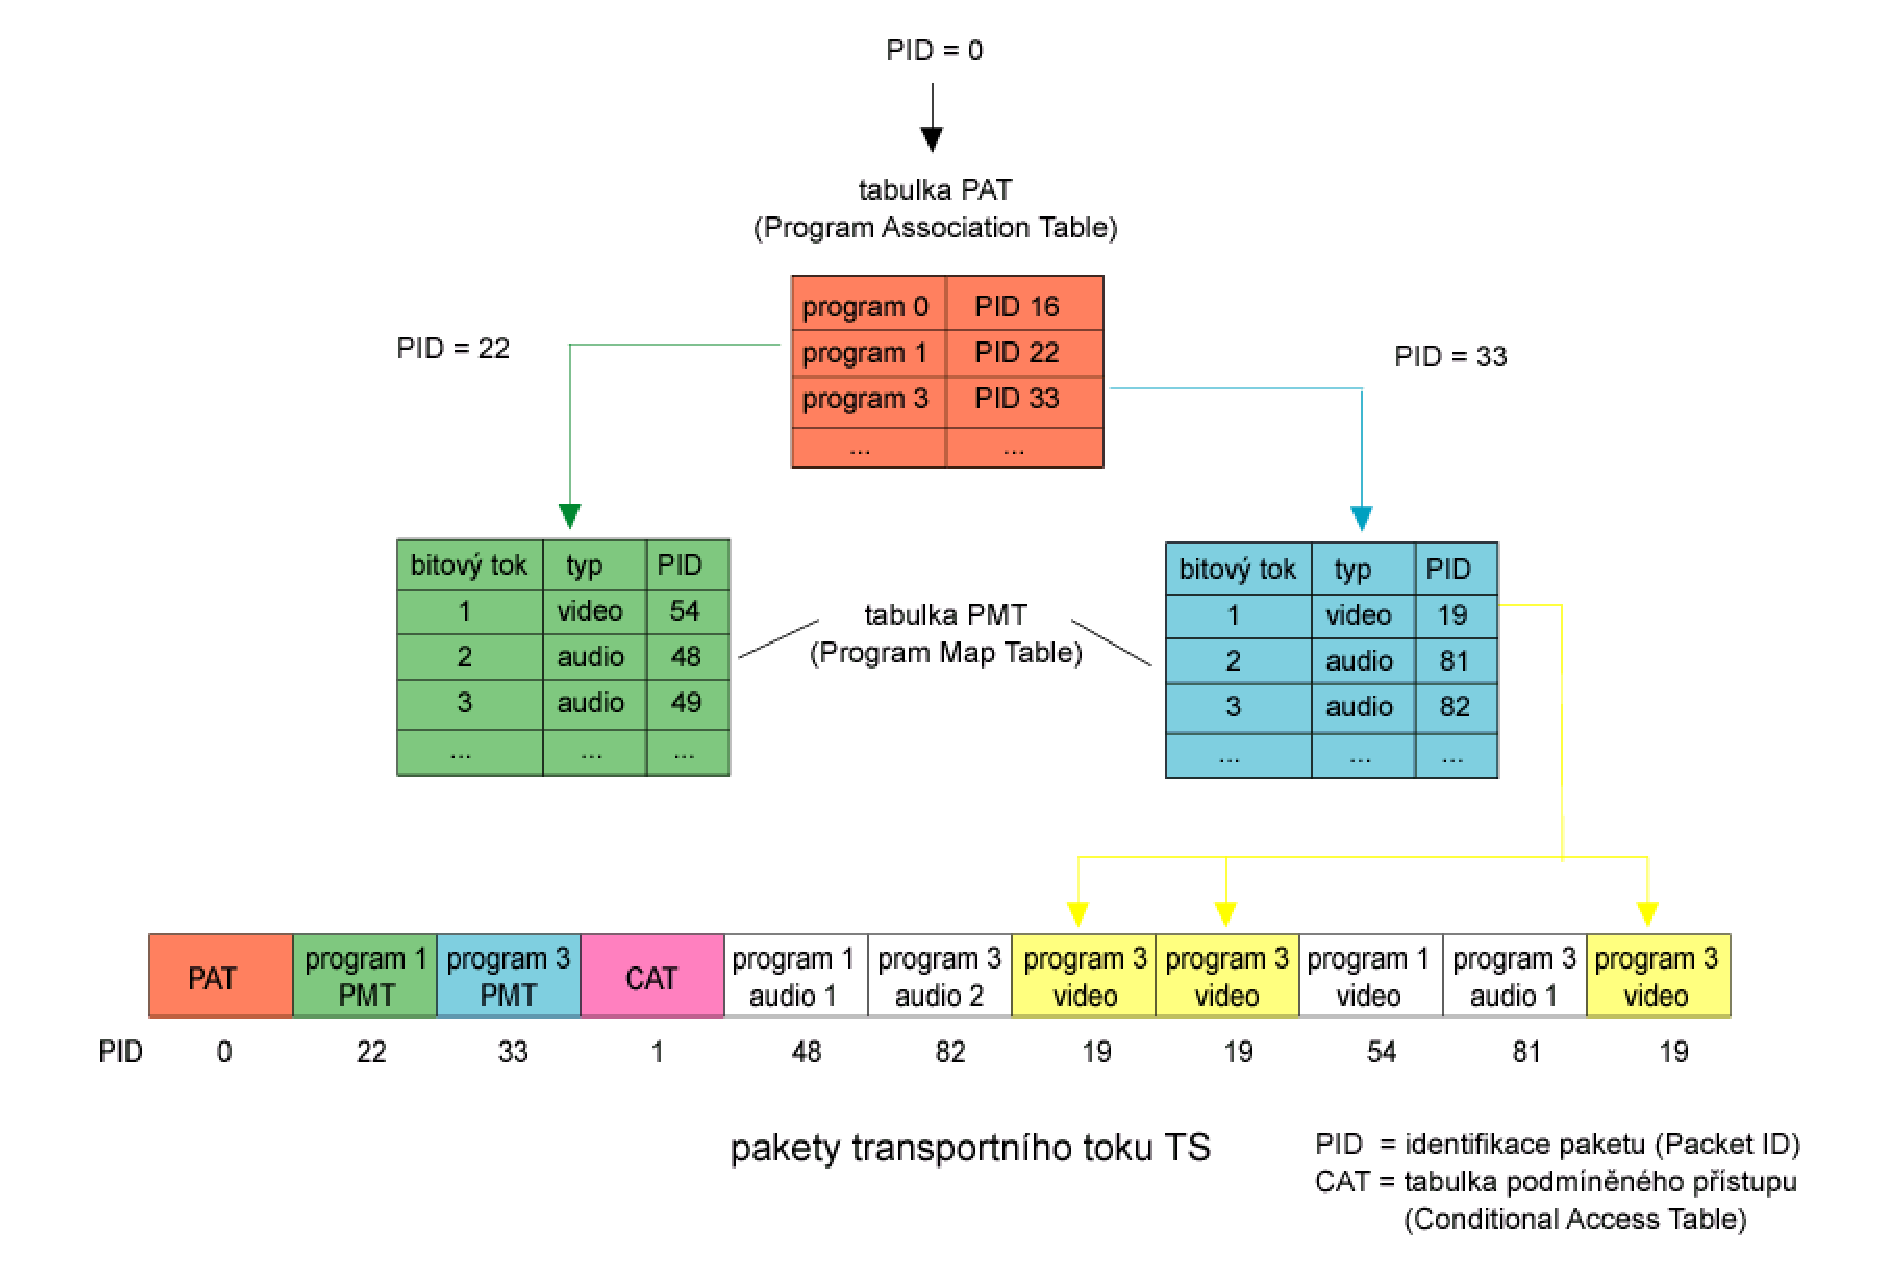
\includegraphics[width=15cm]{images/PATaPMT.eps}
\caption{Tabulky toků v MPEG-2}
\label{fig:PATaPMT}
\end{center}
\end{figure}

\vspace{10pt}

Ještě si také musíme rozhodnout jakou metodu vysílání použijeme.

\vspace{10pt}

Metody vysílání:

\vspace{10pt}

\begin{bf}$Unicast$\end{bf}


\begin{bf}Popis:\end{bf} vysílání pro konkrétní IP adresu


\begin{bf}Výhody:\end{bf} snadná konfigurace pro málo uživatelů, možnost definovat povolené adresy


\begin{bf}Nevýhody:\end{bf} data se posílají tolikrát kolik je uživatelů, značně zatežuje sít

\vspace{10pt}

\begin{bf}$Multicast$\end{bf}


\begin{bf}Popis:\end{bf} vysílání pro skupinu IP adres


\begin{bf}Výhody:\end{bf} do skupiny se klient může přihlašovat a odhlašovat pomocí IGMP paketů, takže dostává data jen z těch stanic, které sleduje.


\begin{bf}Nevýhody:\end{bf} pro funkční a efektivní multicast vysílání je potřeba, aby switche podporovali IGMP snooping, což je mechanismus přeposílání packetů pouze na ty porty, ze kterých přišel přihlašovací paket do dané skupiny, jinak se to šíří v rámci switche jako broadcast.

\vspace{10pt}

\begin{bf}$Broadcast$\end{bf}
   

\begin{bf}Popis:\end{bf} vysílání na úplně všechny IP v síti
 

\begin{bf}Výhody:\end{bf} snadné


\begin{bf}Nevýhody:\end{bf} značné zatížení sítě, data dostávají všichni a ze všech stanic

\vspace{10pt}

Když máme seznam pořadů a přidělíme jim některé multicastove IP adresy, je vhodné vytvořit také statický playlist. Je to obyčejný textový soubor obvykle s příponout .m3u obsahující pro každý pořad takovéto záznamy.

\vspace{10pt}

\begin{small}
\begin{verbatim}
#EXTM3U
#EXTINF:0,CRA_CT1
rtp://@239.194.12.1
...
#EXTINF:0,CRA6_CT1
rtp://@[ff08::701]
...
\end{verbatim}
\end{small}

\vspace{10pt}

\section{VideoLAN Server nebo VideoLAN Client?}

Pro vysílání můžee použít buď VLS nebo VLC. Zásadní rozdíl je ve složitosti a udržovanosti projektu. VLS se již několik let nevyvíjí, VLC už podporuje všechny jeho funkce a nyní i mnohem více.

VLS má složitějsí konfiguraci, je potřeba definovat správně seznam kanálu pro jednotlivé karty v souborech .dvbrc.N. Také neobsahuje integrovany SAP server jako VLC takže je navíc konfigurace SAP serveru a i vlastní vls.cfg je sice přehledný, ale přesto dost náchýlný k chybám při úpravách. Velkou výhodou VLS je při použítí na serverech bez grafického prostředí, protože ani jeho binární balícky nezávisejí na žádných grafických knihovnách.

VLC má mnohem snažší konfiguraci nepodporuje .dvbrc.N soubory (což sice znamená, že nemůžeme definovat pro programy symbolické názvy, ale taky to ušetří práci s vytvářením těchto souborů, pokud se skladba programů v multiplexu častěji mění). Má také integrovaný SAP server, takže je vše schováno přehledně v jednom souboru. Nevýhoda u binárních instalačních balíčků se dá obejít buď překompilováním VLC do balíčku bez podpory X serveru nebo například u distribuce Gentoo je to jen o správné volbě USE flagů při instalaci.

\section{VideoLAN Server}

Open source projekt, který umí vysílat do sítě mnoha různými způsoby a z mnoha různých zdrojů.

\vspace{10pt}

Zdroje:

\vspace{10pt}

statické soubory na disku, nebo nějakém médiu (ve formátu MPEG-1, MPEG-2, MPEG-4),
disky DVD v DVD mechanikách,
digitální satelitní vysílání z DVB-S karet,
digitální pozemní vysílání z DVB-T karet,
přímé přenosy z kamery nebo komprimační karty

\vspace{10pt}

Výstupy:

\vspace{10pt}

na konkrétní IP adresu - unicast
na všechny adresy v určité síti - broadcast
na všechny počítače, které se přihlásí k odběru dané skupiny - multicast
a to vše jak ve variantě IPv4 tak v modernější IPv6

\vspace{10pt}

Hardwarové nároky jsou přibližně Pentium 100 MHz a 32MB RAM pro vysílání jednoho datového toku. Pokud jsou vysílány data ze souborů na lokálním disku, tak je větším omezením čtecí rychlost disku a síťové připojení.

\vspace{10pt}

VLS lze používat jak ve verzi pro MS Windows tak pro Linux. K dispozici jsou i zdrojové kódy.

\vspace{10pt}

Instalační binární i zdrojové balíčky jsou ke stažení na adrese \cite{videolanURL}.
Linuxové distribuce obvykle obsahují předpřipravené instalační balíčky (například Gentoo a Debian mají). 

\vspace{10pt}

Konfigurace VLS
\vspace{10pt}

Tady budeme potřebovat výstup s příkazu scan popsaném v předchozí sekci.

Tento výstup potřebujeme zkonvertovat do formátu konfiguračního souboru pro VLS (.dvbrc). Tyto soubory obsahují na prvních řádcích definici multiplexu a jeho parametrů viz. \ref{tab:mplexy}. Pak každý kanál má nastaveno jméno v parametru NAME a poté v SID je identifikační číslo toku (poslední číslice na výstupu scan).

Takže výsledek vypadá asi takto:

\vspace{10pt}

\begin{small}
\begin{verbatim}
LNB ID 1 TYPE 2
  SAT ID 1 NAME "DVBT-Cra" LNBID 1 FMIN 150000000 FMAX 778000000
    TRANSPONDER ID 1 SATID 1 TYPE 2 FREQ 506000000 BANDWIDTH 0 HP_RATE 2 \
     LP_RATE 6 MODULATION 1 TRANSMISSION_MODE 1 GUARD_INTERVAL 2 HIERARCHY 0
      CHANNEL ID 1 NAME "cra_ct1" SATID 1 TPID 1 SID 1 TYPE 0
      CHANNEL ID 2 NAME "cra_ct2" SATID 1 TPID 1 SID 2 TYPE 0
      CHANNEL ID 3 NAME "cra_ct24" SATID 1 TPID 1 SID 3 TYPE 0
      CHANNEL ID 4 NAME "cra_nova" SATID 1 TPID 1 SID 4 TYPE 0
      CHANNEL ID 5 NAME "cra_praha" SATID 1 TPID 1 SID 18 TYPE 0
      CHANNEL ID 6 NAME "cra_vltava" SATID 1 TPID 1 SID 19 TYPE 0
      CHANNEL ID 7 NAME "cra_ddur" SATID 1 TPID 1 SID 21 TYPE 0
      CHANNEL ID 8 NAME "cra_leonardo" SATID 1 TPID 1 SID 22 TYPE 0
      CHANNEL ID 9 NAME "cra_cesko" SATID 1 TPID 1 SID 23 TYPE 0
\end{verbatim}
\end{small}

\vspace{10pt}

pro České Radiokomunikace 

\vspace{10pt}

a

\vspace{10pt}

\begin{small}
\begin{verbatim}
LNB ID 1 TYPE 2
  SAT ID 1 NAME "DVBT-Cdg" LNBID 1 FMIN 150000000 FMAX 778000000
    TRANSPONDER ID 0001 SATID 0001 TYPE 2 FREQ 674000000 BANDWIDTH 0 HP_RATE 2 \
     LP_RATE 6 MODULATION 1 TRANSMISSION_MODE 1 GUARD_INTERVAL 2 HIERARCHY 0
      CHANNEL ID 1 NAME "cdg_prima" SATID 1 TPID 1 SID 1 TYPE 0
      CHANNEL ID 2 NAME "cdg_top" SATID 1 TPID 1 SID 2 TYPE 0
      CHANNEL ID 3 NAME "cdg_nova" SATID 1 TPID 1 SID 3 TYPE 0
      CHANNEL ID 4 NAME "cdg_ct2" SATID 1 TPID 1 SID 4 TYPE 0
      CHANNEL ID 5 NAME "cdg_ct1" SATID 1 TPID 1 SID 5 TYPE 0
      CHANNEL ID 6 NAME "cdg_cro2" SATID 1 TPID 1 SID 6 TYPE 0
      CHANNEL ID 7 NAME "cdg_ct24" SATID 1 TPID 1 SID 7 TYPE 0
      CHANNEL ID 8 NAME "cdg_cro1" SATID 1 TPID 1 SID 9 TYPE 0
      CHANNEL ID 9 NAME "cdg_proglas" SATID 1 TPID 1 SID 11 TYPE 0
      CHANNEL ID 10 NAME "cdg_e2" SATID 1 TPID 1 SID 19 TYPE 0
      CHANNEL ID 11 NAME "cdg_expres" SATID 1 TPID 1 SID 22 TYPE 0
      CHANNEL ID 12 NAME "cdg_classic" SATID 1 TPID 1 SID 23 TYPE 0
\end{verbatim}
\end{small}

\vspace{10pt}

pro Czech Digital Group.

\vspace{10pt}

Tyto dva soubory pojmenujeme .dvbrc pro první DVB kartu a .dvbrc.1 pro druhou. Soubory uložíme do domovského adresáře uživatele pod kterým budeme chtít VLS spouštět. Pravděpodobně vytvoříme speciálního neprivilegovaného uživatele třeba vls s domovským adresářem například /var/lib/vls.

\vspace{10pt}

Vlastní konfigurační soubor VLS je obvykle /etc/videolan/vls.conf. 

\vspace{10pt}

Na začátku obsahuje společné nastavení jako telnet rozhraní pro správu vls po spuštění. Která myslím nepotřebuje dodatečný komentář.

\vspace{10pt}

\begin{small}
\begin{verbatim}
#
# Nastavení aplikace
#
BEGIN "Vls"
  LogFile       = "/var/log/vls"        # log soubor
  ScreenLog     = "disable"             # logovat na obrazovku
  SystemLog     = "enable"              # logovat do systémového logu
END

#
# Povolené příkazy pro telnetové uživatele
#
BEGIN "Groups"
  monitor       = "help|browse|logout"
  master        = "help|browse|start|resume|suspend|stop \
                   |shutdown|logout|config|program|input|channel|show"
END

#
# Uživatelé pro telnet
#
BEGIN "Users"
  monitor       = "3BcKWoiQn0vi6:monitor"       # heslo nastaveno na 'monitor'
  master        = "JKg2TpPerilnw:master"        # heslo nastaveno na 'bozo'
END

#
# Nastavení telnet rozhraní
#
BEGIN "Telnet"
  Domain        = "Inet4"              # Inet4 nebo Inet6
  LocalAddress  = "127.0.0.1"          # Adresa lokálního rozhraní
  LocalPort     = "9999"               # Použitý port
  Use           = "true"               # Povolit telnet
END
\end{verbatim}
\end{small}

\vspace{10pt}

Dále je obsažena definice zdrojů dat

\vspace{10pt}

\begin{small}
\begin{verbatim}
#
# Zdroje toků dat
#
BEGIN "Inputs"
  dvb0          = "dvb"                 # Video výstup z první DVB karty, 
                                        # odpovídá .dvbrc souboru
  dvb1          = "dvb"                 # Video výstup z druhé DVB karty, 
                                        # odpovídá .dvbrc.1 souboru
END

#
# Konfigurace video vstupů
#
BEGIN "dvb0"                           # Multiplex A CRA
  Frequency = "506000000"              # Frekvence
  DeviceNumber = "0"                   # Zařízení /dev/dvb/adapter<i>
  SendMethod   = "0"                   # 0 - Posílat všechny toky k danému programu, 
                                       # 1 - posílat jen MPEG2 data
  IgnoreTimeout = "1"                  # Ignorovat timeout
  TrickPlay = "normal"                 
END
BEGIN "dvb1"                           # Multiplex B CDG
  Frequency = "674000000"              # Frekvence
  DeviceNumber = "1"                   # Zařízení /dev/dvb/adapter<i>
  SendMethod   = "0"                   # 0 - Posílat všechny toky k danému programu, 
                                       # 1 - posílat jen MPEG2 data
  IgnoreTimeout = "1"                  # Ignorovat timeout
  TrickPlay = "normal"
END
\end{verbatim}
\end{small}

\vspace{10pt}

Definice distribučních kanálů, nejdříve je v Channels seznam distribučních kanálů a pak má každý svou sekci s konfigurací. Na ukázku jsou zobrazeny varianty jak pro použití IPv4 tak IPv6.

\vspace{10pt}

\begin{small}
\begin{verbatim}
#
# Seznam distribučních kanálů
#
BEGIN "Channels"
  mcra_ct1        = "network"
  mcra6_ct1       = "network"
...
END
#
# Konfigurace distribučních kanálů
#
BEGIN "mcra_ct1"               # Program CT1 z multiplexu CRA přes IPv4
  Type      = "multicast"      # Medota vysílání je multicast
  TTL       = "1"              # Dosah vysílání je pouze po nejbližší 
                               # router (pouze vnitřní sít)
  DstHost   = "239.194.12.1"   # Multicastova IP adresa, 
                               # identifikátor multicast skupiny
  DstPort   = "1234"           # Port
  Interface = "eth0"           # Přes které síťové rozhraní chceme posílat data
END
BEGIN "mcra6_ct1"              # Program CT1 z multiplexu CRA přes IPv6
  Domain    = "inet6"          # Typ IPv6
  Type      = "multicast"      # Medota vysílání je multicast
  TTL       = "1"              # Dosah vysílání je pouze po nejbližší 
                               # router (pouze vnitřní sít)
  DstHost   = "ff08::701"      # Multicastova IP adresa, 
                               # identifikátor multicast skupiny
                               # ff08 značí lokální multicast v ramci místní sítě a 
                               # 701 je identifikátor skupiny
  DstPort   = "1234"           # Port
  Interface = "eth0"           # Přes které síťové rozhraní chceme posílat data
END
...

\end{verbatim}
\end{small}

\vspace{10pt}

Spouštění kanálů při startu VLS. Parametry --rtp zajišťuje vysílání synchronizačních údajů společně s UDP datovými pakety a díky tomu pak vysílání jde přehrávat i MPlayerem.

\vspace{10pt}

\begin{small}
\begin{verbatim}
#
# Příkazy po spuštění
#
BEGIN "LaunchOnStartUp"
  command0  = "start cra_ct1 mcra_ct1 dvb0 --rtp"
   # Spuštění programu ČT1 (v .dvbrc musí být přesně cra_ct1) ze zdroje dvb0 
   # přes distribuční kanál mcra_ct1
  command1  = "start cra_ct1 mcra6_ct1 dvb0 --rtp"   
   # Spuštění programu ČT1 (v .dvbrc musí být přesně cra_ct1) ze zdroje dvb0 
   # přes distribuční kanál mcra6_ct1
...
END

\end{verbatim}
\end{small}

\vspace{10pt}

VLS je skvělý program pro serverové použití, nepotřebuje grafické knihovny, jeho konfigurace je přehledná. Vývoj jde ale rychleji kupředu v podobném projektu ze stejné dílny, který je zároveň jak klientským prohlížečem tak streamovacím serverem. Tento produkt se jmenuje VideoLAN Client VLC.

\vspace{10pt}

\section{Mini SAP server}

Opět open source projekt, SAP(Session Announcment Protocol) je protokol pro oznamování změn ve skladbě vysílání. Uživatelé mohou zvolit 2 přístupy. Buď použíjí staticky vygenerovaný soubor .m3u, který obsahuje seznam kanálů, které v síti vysíláme, ale při každé změně musíme aktualizovat .m3u soubor a uživatelé si musí stáhnout někde aktuální verzi. Druhá možnost je použít tohoto programu, který běží na serveru obvykle tom který vysílá. A v jeho konfiguraci je také seznam kanálů, které vysíláme, ale pokaždé když provedeme změnu, tak se tato změna projeví ihned i všem uživatelům, kteří mají nastaveno používání playlistu ze SAP služby.

\vspace{10pt}

SAP server tyto informace posílá také pomocí multicast vysílání, podporuje také jak IPv4 tak IPv6 variantu.

\vspace{10pt}

Mini-SAP-server lze provozovat pod operačním systémem Linux a Mac OS X. 

\vspace{10pt}

Instalace je snadná, po stažení zdrojových kódů by měla stačit obvyklá sekvence ./configure \&\& make \&\& make install. A možná bude k dispozici i instalační balík přímo z distribuce.

\vspace{10pt}

Konfigurace je opět celkem přímočará, v souboru /etc/sap.cfg má každý kanál takovou sekci: 

\vspace{10pt}

\begin{small}
\begin{verbatim}
[program]
type=rtp
name=CRA CT1
user=Masarka
machine=zeus.mk.cvut.cz
site=http://dvbgrab.mk.cvut.cz/stream
address=239.194.12.1
port=1234
program_ttl=32
program_ipversion=4
playlist_group=Masarka
\end{verbatim}
\end{small}

\vspace{10pt}

Mini SAP Server je velmi snadno použitelný a pro uživatele velmi pohodlný doplněk vysílání. VLC má vysílání SAP informací dokonce zabudováno v sobě. 

\vspace{10pt}

\section{VideoLAN Client}

Další projekt s otevřeným kódem, který podporuje mnoho platforem: Linux, Windows, Mac OS X, BeOS, *BSD, Solaris, Familiar Linux, Yopy/Linupy and QNX. VLC nepracuje na Mac OS 9 a pravděpodobně ani nikdy nebude.

\vspace{10pt}

Umí přahrávat:
soubory z disků a mechanik (formáty MPEG-1, MPEG-2, MPEG-4/DivX apod.)
DVD disky, VCD soubory
ze satelitních/pozemních karet digitálního vysílání DVB-S/DVB-T
z analogových karet přes rozhraní v4l(video for linux)

\vspace{10pt}

Umí také ale vysílat stejně jako VLS.

\vspace{10pt}

Instalace je velmi snadná. K dispozici jsou instalační balíky pro mnoho operačních systémů.

\vspace{10pt}

Konfigurace klienta obecně není potřeba. 

\vspace{10pt}

Trošku pohodlí může přidat vytvoření zástupce/skriptu, který při spuštění načte námi používaný playlist z .m3u souboru, nebo zapne podporu získávání playlistu ze SAP událostí. Klienti si uloží staticky playlist do svého domovského adresáře jako .vlc.m3u a pak do definice Cíl v zástupci ve windows resp. do nějakého startovacího skriptu v linuxu přidají parametry. VLC pak po startu hned obsahuje použitelný playlist a po nějaké prodlevě se doplní ještě SAP playlist.

\vspace{10pt}

\begin{small}
\begin{verbatim}
C:\Program Files\VideoLAN\vlc.exe -S sap %%HOMEPATH%%/.vlc.m3u
resp.
/usr/bin/vlc -S sap ~/.vlc.m3u
\end{verbatim}
\end{small}

\vspace{10pt}

Konfigurace VLC pro použití na vysílání do sítě

\vspace{10pt}

Vše je v jednom souboru, který uložíme například do /etc/videolan/vlm/vlm.cfg.

\vspace{10pt}

\begin{small}
\begin{verbatim}
# Vytvoření nového zdroje dat
new CRA broadcast enabled

# Nastavíme typ zdroje na DVB
setup CRA input dvb:

# Nastavení DVB parametrů viz tabulka.
setup CRA option dvb-adapter=0
setup CRA option dvb-frequency=506000000
setup CRA option dvb-bandwidth=8
setup CRA option dvb-transmission=8
setup CRA option dvb-guard=8
setup CRA option dvb-hierarchy=-1
setup CRA option dvb-modulation=64

# Chceme data nechávat v transport streamu a 
# posílat je po jednotlivých programech
setup CRA option ts-es-id-pid

# Seznam identifikačních čísel programů, které nás zajímají
setup CRA option programs=1,2,3,4,5,10,11,12,13,14,15,16,1000

# Nastavení výstupů

# Použijeme modul duplicate, který z multiplexu vybere toky 
# odpovídající programu podle klauzule select a ty pošle i
# do modulu std který je definován v klauzuli dst

# std modul nastavíme pro typ vysílání rtp, mux=ts znamená 
# nekonvertovat, v url je multicastová IP a port

# sap zajistí vysílání SAP událostí pro daný program, 
# group a name pak udávají jak se bude program
# zobrazovat v klientu po povoleni SAP playlistu

setup CRA output #duplicate
{
dst=std{access=rtp,mux=ts,url=239.194.12.1:1234, \
  sap,group="Masarka-CRA",name="CT1"},select="program=1"
,dst=std{access=rtp,mux=ts,url=239.194.12.2:1234, \
  sap,group="Masarka-CRA",name="CT2"},select="program=2"
,dst=std{access=rtp,mux=ts,url=239.194.12.3:1234, \ 
  sap,group="Masarka-CRA",name="CT24"},select="program=3"
,dst=std{access=rtp,mux=ts,url=239.194.12.4:1234, \
  sap,group="Masarka-CRA",name="CT4"},select="program=4"
,dst=std{access=rtp,mux=ts,url=239.194.12.5:1234, \
  sap,group="Masarka-CRA",name="Nova"},select="program=5"
,dst=std{access=rtp,mux=ts,url=239.194.12.6:1234, \
  sap,group="Masarka-CRA",name="CRO1"},select="program=10"
,dst=std{access=rtp,mux=ts,url=239.194.12.7:1234, \
  sap,group="Masarka-CRA",name="CRO2"},select="program=11"
,dst=std{access=rtp,mux=ts,url=239.194.12.8:1234, \
  sap,group="Masarka-CRA",name="CRO3"},select="program=12"
,dst=std{access=rtp,mux=ts,url=239.194.12.9:1234, \
  sap,group="Masarka-CRA",name="CRO4"},select="program=13"
,dst=std{access=rtp,mux=ts,url=239.194.12.10:1234, \
  sap,group="Masarka-CRA",name="Ddur"},select="program=14"
,dst=std{access=rtp,mux=ts,url=239.194.12.11:1234, \
  sap,group="Masarka-CRA",name="Leonardo"},select="program=15"
,dst=std{access=rtp,mux=ts,url=239.194.12.12:1234, \
  sap,group="Masarka-CRA",name="Cesko"},select="program=16"
,dst=std{access=rtp,mux=ts,url=239.194.12.13:1234, \
  sap,group="Masarka-CRA",name="MHP"},select="program=1000"
}
\end{verbatim}
\end{small}

\vspace{10pt}

Spouštění po startu zajistíme například přidáním spouštěcího skriptu do /etc/init.d/vlm, který v podstatě přečte konfiguraci například z /etc/sysconfig/dvb.

\vspace{10pt}

\begin{small}
\begin{verbatim}
VLM_CONFIG_FILE=/etc/videolan/vlm/vlm.cfg
VLM_LOG_FILE=/var/log/vlm.log
VLM_TELNET_PORT=7777
VLM_TELNET_PASSWORD=password
\end{verbatim}
\end{small}

\vspace{10pt}

a pak spustí VLC v režimu VLM (VideoLAN Manager) pouze s telnetovým rozhraním.

\vspace{10pt}

\begin{small}
\begin{verbatim}
VLCSERVER=/usr/bin/vlc
daemon --user vlc "$VLCSERVER" -d -vvv --logfile $VLM_LOG_FILE --file-logging \
  --vlm-conf $VLM_CONFIG_FILE --intf telnet --telnet-port $VLM_TELNET_PORT \
  --telnet-password $VLM_TELNET_PASSWORD 2> /dev/null
\end{verbatim}
\end{small}

\vspace{10pt}

Kontrolu zda vše správně běží můžeme provést přihlášením na telnet \begin{small}\begin{verbatim}telnet server port\end{verbatim}\end{small} a zadáním příkazu \begin{small}\begin{verbatim}show\end{verbatim}\end{small}. Objeví se seznam zdrojů a jejich stav. Zadáním \begin{small}\begin{verbatim}show název\end{verbatim}\end{small}, zobrazíme podrobnější údaje pro daný zdroj a pomocí \begin{small}\begin{verbatim}control název stop\end{verbatim}\end{small} ho můžeme například zatavit.

\vspace{10pt}

Nyní je předpokládám vidět rozdíl v jednoduchosti úprav konfigurace VLS a VLC. Například přidání nového televizního v kanálu je ve VLC jeden nový řádek, ve kterém nastavíme select na zjištěné ID kanálu a zvolíme multicast IP adresu a skupinu a název pro SAP. U VLS přidání jednoho kanálu, znamená přidání řádku do odpovídajícího .dvbrc souboru. Odteď si musíme pamatovat jaký název jsme mu přiřadili. V souboru vls.conf přidáme nový distribuční kanál a zvolíme multicast adresu a port. Nyní už si musíme pamatovat jak název kanálu v .dvbrc, tak název distribučního kanálu ve vls.conf a IP adresu a port. To využijeme při přidávání nového kanálu do automatického spouštění po startu. IP adresu a port použijeme ještě při úpravě konfigurace SAP serveru.

\vspace{10pt}

\section {MPlayer}

MPlayer je dalším přehrávačem, který můžeme použít pro příjem vysílání z lokální sítě. A zároveň je nejoblíbenějším Linuxovým video přehrávačem. Podporuje velmi mnoho různých zdrojů v mnoha formátech a samozřejmě také umí přijímat multicastové vysílání z lokální sítě. Jedinou podmínkou je dodržení protokolu vysílání rtp:// místo výchozího udp://. Pohodlné je vytvoření souštecího skriptu pro každý televizní kanál zvlášť.

\vspace{10pt}

Instalace je snadná, buď použijeme distribuční balík, nebo opět kompilací zdrojových kódů ze stránek \cite{mplayerURL}. 

\vspace{10pt}

Konfigurace.. spouštěcí skripty mohou vypadat například takto:
mplayer -framedrop rtp://239.194.12.1:1234 
pro příjem vysílání z multicastové adresy 239.194.12.1. A skript pak pojmenujeme například tv\_ct1.

\vspace{10pt}

MPlayer je dalším pohodlným přehrávačem, který ale nemá tak jednoduché a přehledné grafické prostředí a nepodporuje SAP playlist.

\vspace{10pt}


\chapter{Příjem multicastového vysílání z vnější sítě}

Na Internetu je dostupných i mnoho dalších televizních kanálů, které jsou vysílány pro veřejnost. Příjem je ale problematický, protože musí být zaručeno směrování multicastu z veřejného Internetu až do naší sítě. Je třeba vyřešit kompatibilitu multicastových démonů na routerech založených na Linuxu s Cisco routery. Tak aby mezi v naší síti a v síti poskytovatele připojení byla na každém sousedním routeru spuštěna služba pro směrování multicast dat. Případně lze vytvořit tunel, kterým jsou některé multicastové skupiny vysílány jako klasické unicast pakety. Směrování multicast paketů a správu skupin obvykle poskytuje pim démon na cisto routerech, na linuxových pak například pimd nebo mrouted.

\vspace{10pt}

Pro operační systém Linux se nejčastěji používají 2 multicastové směrovací démoni pimd a mrouted. Bohužel se už nevyvíjí a jejich současné verze rozhodně nejsou dokonalé.

\vspace{10pt}

\textbf{PIMd}

\vspace{5pt}

Poslední verze která se používá je alpha verze z roku 1999. Podporuje směrovací protokol DVMRP a MOSPF. Hodí se pro více využité multicastové skupiny nebo pro sítě s velkým přenosovým pásmem.

\vspace{10pt}

Pokud jsou skupiny využívané zřídka tak toto schéma přestává být efektivní. Proto vznikla odnož pim démona:

\vspace{10pt}

\textbf{PIM-SM}

\vspace{5pt}

Pim démon v sparse módu. Udržuje tabulku odběratelů a zdrojů určité skupiny a podle toho vytváří distribuční stromy. Kořen distribučních stromů se nazývá "Rendezvous Point".

\vspace{10pt}

Implementace pim démona s otevřeným kódem

Zastaralý: \textbf{Pimd USC site} (samostatný PIM-SM + úprava jádra systému)

Zastaralý: \textbf{PIM-SM GateD} implmentace od ISI.

\textbf{PIM-DM GateD} implementace z Oregonské univerzity

\textbf{Pimd-dense} samostatná implementace z Oregonské univerzity

\textbf{PIM-SM} implementace z XORP projektu (implementace software směrovačů s otevřeným kódem)

\vspace{10pt}

Více viz \cite{pimdURL}.

\vspace{10pt}

\textbf{MROUTEd}

\vspace{5pt}

Poslední používaná verze je beta z roku 1999. Mrouted implementuje také DVMRP směrovací protokol. Podporuje také tunely skrz směrovače, které nepodporují multicast. Více viz \cite{mroutedURL}.


\chapter{Testování}

V rámci předmětu Styk člověka s počítačem jsem provedl i test tohoto systému.

\vspace{10pt}

Když byl systém provozován přibližně rok na Masarykově koleji a měl registrováno cca 120 uživatelů, tak jsem rozeslal všem registrovaným neformální žádost. Žádost byla prvním krokem, chtěl jsem získat přehled, jaké se vyskytují chyby a nejasnosti v uživatelském rozhraní. 

\vspace{10pt}

Systém je zaměřený převážně na studentské prostředí, proto nebylo do testu zařazeno více osob včetně osob, které systém nikdy nepoužili.

\vspace{10pt}

Na email odpovědělo sice pouze asi 10 osob, přesto byly nalezeny, některé vhodné vylepšení:

\vspace{10pt}

\section{Připomínky a reakce na ně}

\begin{bf}Připomínka:\end{bf} Všechny díly seriálu by mělo být možno objednat jedním tlačítkem.

\begin{bf}Reakce:\end{bf} Nyní je možnost vyhledat v televizním programu podle názvu, takže všechny díly daného seriálu lze nalézt podle zadané části názvu, a pak objednat snadno a rychle v seznamu výsledků hledání. To je univerzálnější a navíc není potřeba z programu detekovat co je a co není seriál a také není třeba zaznamenávat tyto seriálové požadavky mimo rozsah programu, který známe předem. (když objednám seriál který má 4 díly v programu, který už je načten a další 4 v programu, který se načte až při příští aktualizaci, tak bych musel udržovat další tabulku ?dlouhodobých požadavků?.

\vspace{10pt}
 
\begin{bf}Připomínka:\end{bf} Odkazy na nahrané pořady uveřejňovat po přihlášení přímo na stránkách. 

\begin{bf}Reakce:\end{bf} Nyní se odkaz odešle po nahrání jen na emaily uživatelů, kteří si to objednali. Pokud email smažou a odkaz si neuloží tak nemají možnost se k záznamu dostat (kontrola IP adresy uživatele a generovaná část názvu pořadu). Tato část bude po několika úpravách implementována, protože značně zjednoduší použití systému a seznam nahraných pořadů pro jednotlivé uživatele již je na webu k dispozici, stačí přidat název souboru pro jednotlivé požadavky, který se vyplní po úspěšném nahrání a na webu přidat do seznamu sloupec s odkazem.

\vspace{10pt}

\begin{bf}Připomínka:\end{bf} Uživatelé si občas neuvědomují, že zadání správného mailu je podmínkou pro použití systému. Při registraci zadají nějakou hloupost a pak marně čekají jak se dozví o úspěšném nahrání pořadu.

\begin{bf}Reakce:\end{bf} Tady by mohlo stačit výraznější varování v registračním formuláři, protože bohužel souhrnné informace o tom jak to celé funguje (půl strany textu na úvodní stránce) asi nikdo nečte.

\vspace{10pt}

\begin{bf}Připomínka:\end{bf} Jeden člověk si stěžoval, že mu na webu vadí seznam nahrávek všech uživatelů a přihlášeného uživatele. Prý by to mělo patřit do administrativní části webu.

\begin{bf}Reakce:\end{bf} S tím nesouhlasím, protože pokud nějaký pořad nestihnu objednat, tak můžu například využít kontaktu (email,icq,jabber) na osobu ze seznamu, která si to objednala a zkusit se s ni domluvit na zpřístupnění.

\vspace{10pt}

\begin{bf}Připomínka:\end{bf} Stejnému člověku přišlo, že hlavní stránka + 6 podstránek je zahlcení uživatele. 

\begin{bf}Reakce:\end{bf} S tím také nesouhlasím, protože já jako uživatel a spousta dalších tyto podstránky používá a například seznam uživatelem nahraných pořadů získá s doplněním odkazů na jejich stažení další velký význam. Další výhodou zobrazovaného seznamu je lepší přehled uživatele, protože počet objednaných nahrávek za měsíc je omezen.

\vspace{10pt}

\begin{bf}Připomínka:\end{bf} Lepší vysvětlení co znamená ?nagrabovat? a ?nagrabovat do TS?. 

\begin{bf}Reakce:\end{bf} V úvodních informacích je napsáno, že po vybrání pořadu se objedná nahrávka s komprimací do MPEG4. Pokud uživatel chce provádět na nahrávce další úpravy je pro něj výhodnější nahrávku nekomprimovat a zanechat ve formátu MPEG2-TS. Protože není na seznamu pořadů moc místa, tak je uveden pouze odkaz ?nagrabovat? a po potvrzení dialogu "Doopravdy chcete nahrát pořad abc?? se odkaz změní na ?zrušit grab? a vedle se zobrazí ?do TS?, čímž se zruší objednávka buď úplně nebo se zruší její komprimace (využitelné pro cca 5\% uživatelů). Navrhované řešení bylo nahradit dialog s ?ANO?, ?NE? kompletní novou podstránkou s formulářem, který by zobrazoval detail zvoleného pořadu a obsahoval i popis co je MPEG4, MPEG-TS a jak se o nahrání uživatel dozví. Na formuláři by pak mohli být tlačítka ?Zruš grab?, ?Grabuj do MPEG4?, ?Grabuj do MPEG-TS? a ?Storno?. Toto by sice bylo možné, ale na původním způsobu jsem oceňoval rychlost použití. Klik na název pořadu, enter na klávesnici pro volbu ?ANO? a už bylo objednáno. Takhle než se zobrazí formulář se spoustou opakujících se informací (popis formátů, způsob doručení odkazu pro stažení), zvolit správné tlačítko a počkat na opětovné vykreslení celého televizního programu bude velmi zdržující.

\vspace{10pt}

\begin{bf}Připomínka:\end{bf} Jeden uživatel si také stěžoval na nemožnost změnit si dodatečně email adresu. 

\begin{bf}Reakce:\end{bf} Tato možnost tam je ?schována? v menu nastavení. Bohužel nenapadá mě výstiženější název pro podstránku, kde se nastavují parametry účtu.

\vspace{10pt}

\section{Vyhodnocení implementovaných připomínek - anketa}

Pro zjištění jak uživatelé hodnotí provedené změny jsem opět rozeslal na seznam registrovaných členů email s žádostí o vyplnění krátké ankety, kterou jsem začlenil do webového rozhraní DVBgrabu. Každá odpověd se zkládala z číselného ohodnocení 1=Rozhodně ANO až 5=Rozhodně NE a textového komentáře.

\vspace{10pt}

Anketa dopada takto:

\vspace{10pt}

\begin{bf}Otázka:\end{bf}: Odkazy na stažení grabů budou nyní dostupné přímo z menu "Moje graby". Je tato vlastnost pro Vás přínosná?

\begin{bf}Odpovědi:\end{bf} Všichni novou možnost uvítali, pouze 2 ohodnotili 4, z toho jeden byl "věčným nespokojencem".

\vspace{10pt}

\begin{bf}Otázka:\end{bf} Nyní můžete objednávat seriály přes vyhledání v tv programu a v seznamu výsledků, rychlým klikáním na jednotlivé díly. Chtěli byste mít i možnost objednat všechny díly seriálu jedním tlačítkem, které by ale dost problematicky poznávalo co je a co není seriál a také by muselo složitě řesit objednávání seriálů na dobu delší než na kolik se načítá tv program. Potřebujete tuto funkčnost?

\begin{bf}Odpovědi:\end{bf} Opět se většina shodla ohodnocení 4-5 a "věčný nespokojenec" by požadoval i tuto funkci.

\vspace{10pt}
						
\begin{bf}Otázka:\end{bf} Je ze současných textů už zřejmé, že správný email je podmínkou použitelnosti DVBgrabu?

\begin{bf}Odpovědi:\end{bf} Všichni potvrdili, že situace už je napravena, "věčně nespokojeny" opět doplnuje, že s odkazy na graby z menu je už mail jenom doplnkovou podmínkou.
							
\vspace{10pt}

\begin{bf}Otázka:\end{bf} Je ze současných textů už zřejmé co myslím MPEG4 a transport stream TS a co je výchozí volbou při grabování?

\begin{bf}Odpovědi:\end{bf} Vyhodnocení je sporné, ale spíše pozitivní reakce, součástí komentářů byly i 2 dobré nápady na vylepšení.
							
\vspace{10pt}

\begin{bf}Otázka:\end{bf} Příjdou vám menu "seznam mých, plánovaných, hotových grabů" zbytečná nebo je občas rádi využíváte? Takže tyto menu zachovat nebo ne?

\begin{bf}Odpovědi:\end{bf} Všichni dotázaní požadují zachování jen "věčně nespokojený" přidává, že je nepotřebuje.
							
\vspace{10pt}

\begin{bf}Otázka:\end{bf} Všimli jste si v menu volby "Nastavení" a hodila se Vám?	

\begin{bf}Odpovědi:\end{bf} Opět pozitivní odezva.
						
\vspace{10pt}

\begin{bf}Otázka:\end{bf} Chybí Vám tu nějaká funkce? Případně do komentáře napište jaká.

\begin{bf}Odpovědi:\end{bf} Nikdo nic nepostrádal.
				
\vspace{10pt}

\begin{bf}Otázka:\end{bf} Libovolný vzkaz tvůrci DVBgrabu, náměty na vylepšení atd.

\begin{bf}Odpovědi:\end{bf} Pár slov chvály a několik neuskutečnitelných návrhů.

\vspace{10pt}

\section{Vyhodnocení ankety}

Uživatelé byli dotazování na konkrétní body a konkrétní funkce, protože možnost vyjádřit se k systému jako celku měli v prvním kole emailů. Také se projevil ?věčný nespokojenec?, který nebyl spokojen vcelku s ničím, ale vzhledem k tomu, že svým názorem značně vyčníval mimo průměr, mohl být jeho názor vyřazen.

\vspace{10pt}

\section{Závěr}

I přes účast pouze několika málo uživatelů se podařilo dát dohromady několik návrhů na vylepšení, které mohou daný systém zlepšit, zpřehlednit a urychlit, proto si myslím, že testování se rozhodně vyplatilo. Navíc když bylo provedeno touto formou, tak nevyžadovalo žádné velké úsilí navíc. Také bylo objeveno několik drobných chyb v programu.

\vspace{10pt}

Kdyby byl test proveden na ruznorodém vzorku uživatelů (nejenom studenti technické školy) mohly se objevit i úplně jiné problémy, ale toto jsem netestoval, protože zatím nehodlám uveřejnit systému i pro tyto cílové skupiny uživatelů.

\chapter{Závěr}
Aplikace DVBgrab je v současné době úspěšně používána v minimálně 5 instalacích převážně na kolejích ČVUT. 

Za účelem zajištění jejího dalšího zlepšování jsem ji zaregistroval na portálu opensource projektů http://sourceforge.net, kde byla komisí přijata a tak je od 8. prosince 2006 dostupná její instalace ze stránek http://dvbgrab.sourceforge.net. Na servery sourceforge byl také přesunut vývojový repozitář pro verzovací systém subversion.

V budoucnu by se dalo implementovat navrhované vystřihování reklamy a získávání televizního programu přímo z MPEG-2 signálu, místo komplikovaného načítání z webových zdrojů.


\cleardoublepage

%*************************************************************************
\bibliography{dp_bibliography}
%bibliographystyle{plain}
\bibliographystyle{abbrv}

\cleardoublepage

%*************************************************************************
\appendix
\chapter{Instalace a údržba}

\vspace{10pt}

Aplikace lze provozovat jako 2 oddělené celky, kterým můžeme říkat frontend a backend.

\vspace{10pt}

\textbf{Frontend}

Je rozhraní mezi aplikací a uživatelem, v tomto případě tedy webová aplikace běžící na Apache serveru s PHP modulem. Na stejném serveru může běžet i databáze.

\vspace{10pt}

\textbf{Backend}

Je ta část aplikace, která běží na pozadí a zajišťuje vlastní vyhotovování nahrávek. Ze serveru, kde běží backend, se také poté distribuují výsledky. Pokud bychom neměli dostatek místa, je možné aplikaci dále rozdělit na další server, který by se staral o distribuci a nahrávky by se po uložení ukládaly na distribuční server třeba pomocí NFS sdílení. Naopak pokud budeme chtít, může běžet backend na stejném serveru jako frontend.

\vspace{10pt}

\begin{figure}[ht]
\begin{center}
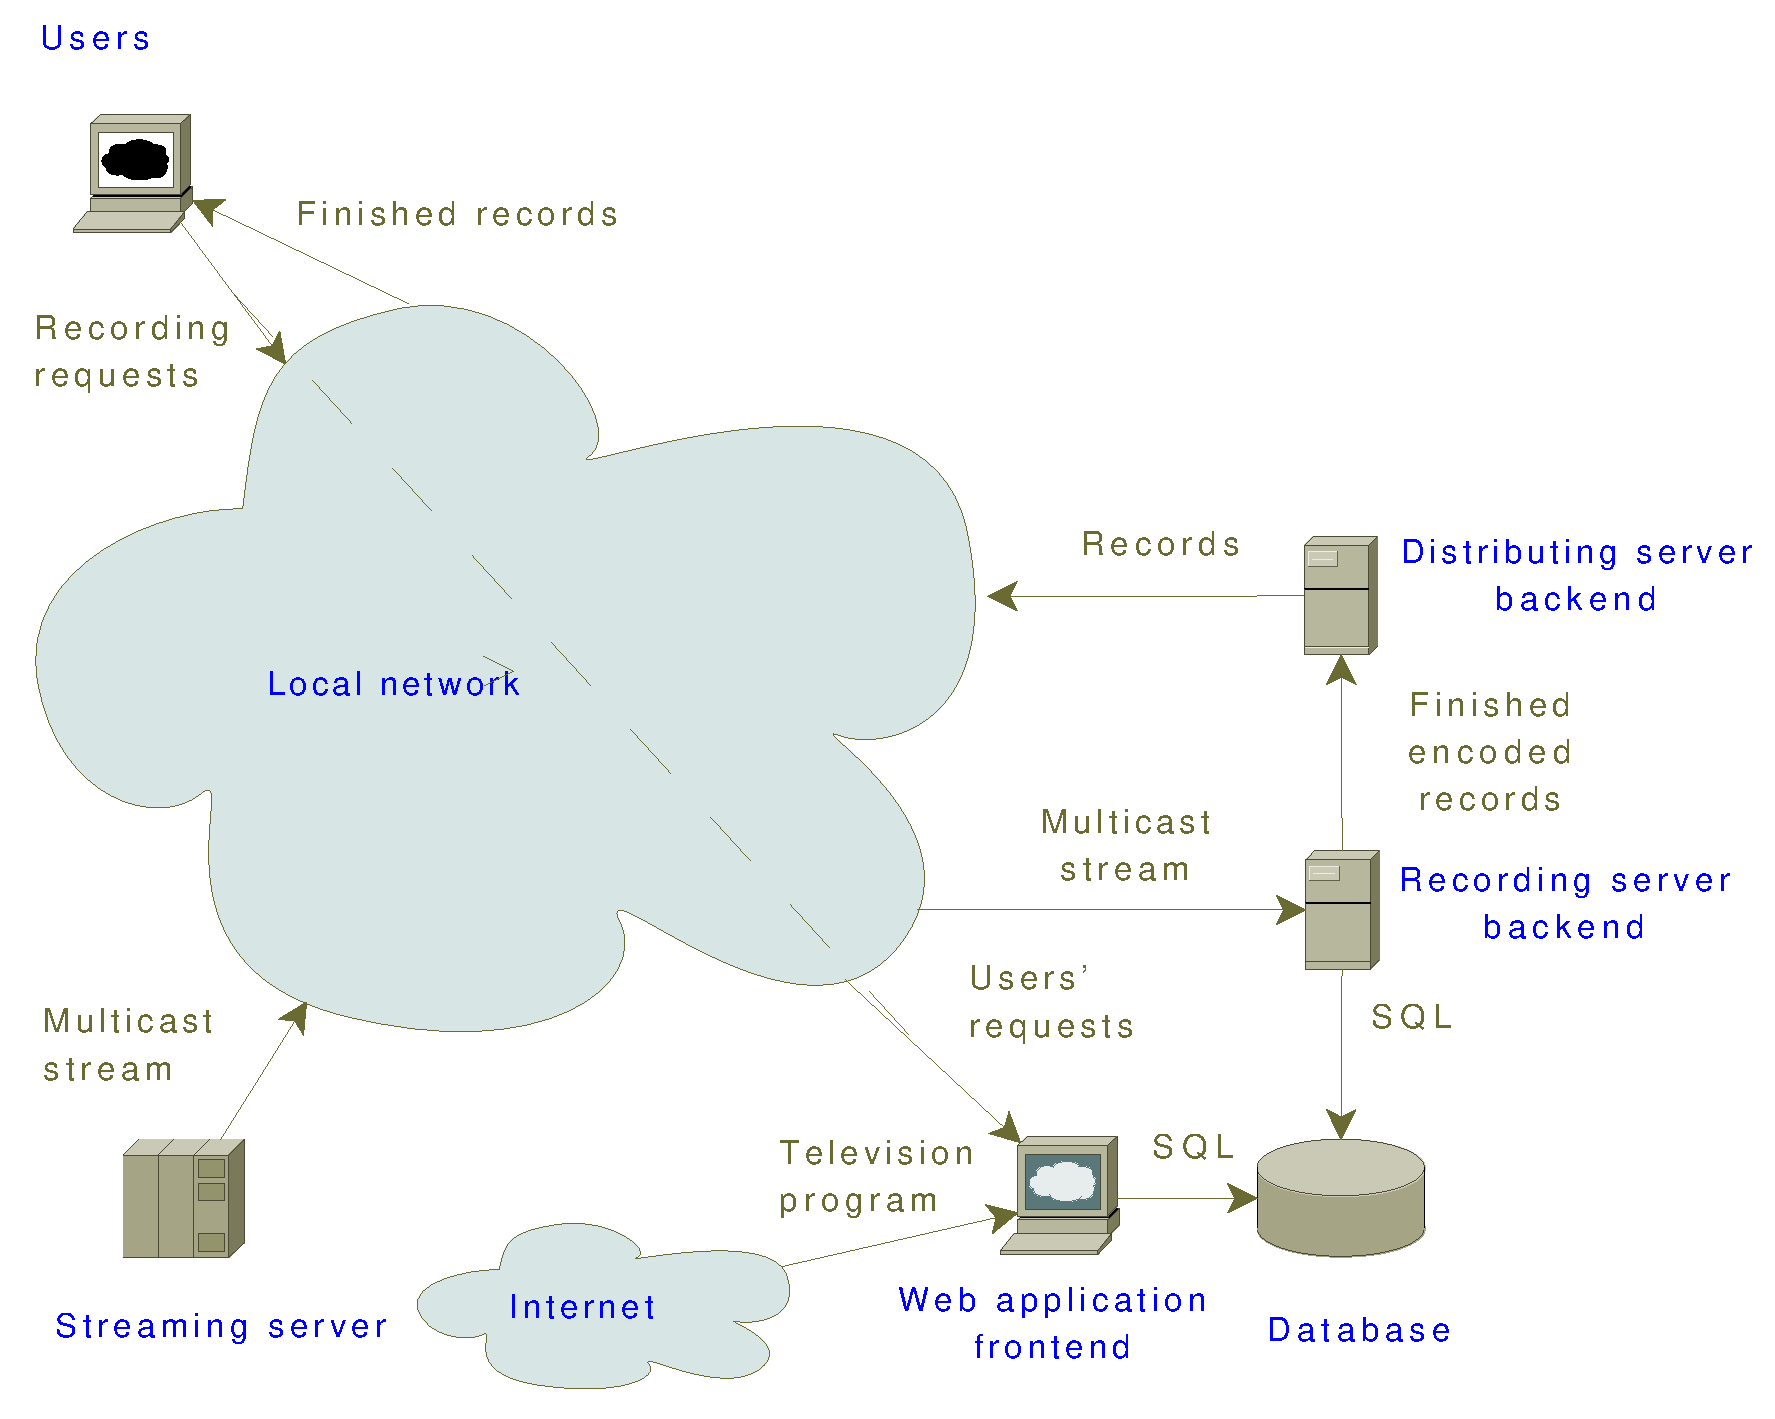
\includegraphics[width=15cm]{images/dvbgrab.eps}
\caption{Komponenty DVBgrabu}
\label{fig:dvbgrab}
\end{center}
\end{figure}

\section{Potřebné knihovny a pomocné programy}

\vspace{10pt}

\textbf{Apache}

Apache jako webový server budeme potřebovat jak na backend tak na frontend serveru.
Minimálně pro backend server je dobré použít buď verzi 1.x nebo až 2.2, protože verze 2.0 měla problémy se soubory většími nez 2GB, které jako graby často vznikají.

\vspace{10pt}

\textbf{PHP}

Na webovém serveru je potřeba modul do apache. Na záznamovém stačí PHP interpret přístupný z příkazového řádku. Obvykle instalace stejně obsahuje oba. Aplikace byla otestována jak na PHP verze 4 tak 5, v PHP musí být povoleny některé rozšíření viz. dále.

\vspace{10pt}

\textbf{php-pear-Log}

Logovací systém, obdoba log4j pro Javu. Je potřeba na obou serverech a jsou přes něj zapisovány veškeré záznamy do logovacích souborů. Logovací soubory se používají 4 a jsou v podadresáři log.

dvbgrab.log - obecné hlášky systému.

dvbgrab.log.sql - veškerý SQL kód, který je volán.

dvbgrab.log.sys - veškeré příkazy operačního systému, které jsou volány z PHP.

dvbgrab.log.clean - logování výstupu z údržbového skriptu.

Logování SQL a systémových příkazů může generovat poměrně velké logy, proto by mělo být po odladění aplikace vypnuto v dolib.inc.php.

\vspace{10pt}

\textbf{php-json}

Podpora pro JSON (JavaScript Object Notation) do PHP. JSON je použit pro dotazy na detail televizního pořadu nebo grabu v seznamu grabů. Je to alternativní notace, která je vrácena na volání XMLHttpRequestu z javascriptu. Toto rozšíření usnadňuje generování JSON odpovědi ve skriptu, který z databáze detail načítá a zpracování přijaté odpovědi ve webové stránce.

\vspace{10pt}

\textbf{php-adodb}

Knihovna pro abstraktní přístup k různým databázím. Všechna volání do databáze překládá ze své syntaxe do syntaxe použitého databázového stroje.

\vspace{10pt}

\textbf{XMLTV}
Pokud chcete použít XMLTV modul pro načítání televizního programu, bude potřeba nainstalovat tento balík. Buď v něm přímo najdete stahovací skript pro požadované programy, nebo se bude hodit alespoň skript tv\_sort.

\vspace{10pt}

\textbf{Databáze}

DVBgrab by měl fungovat s libovolnou databází, která je podporována v adodb. Otestovaný je na postgresql a mysql, také skripty pro založení databáze jsou připraveny v syntaxi pro mysql a postgresql.

\vspace{10pt}

\section{Stažení DVBgrabu}

\vspace{10pt}

DVBgrab je dostupný na na sourceforge.net. K dispozici jsou jak jednotlivé uveřejněné verze, tak čtení z vývojového repozitáře subversion.

Odkaz na jednotlivé verze naleznete na stránkách projektu http://dvbgrab.sourceforge.net/.

Pro export z repozitáře subversion použijte následující:

\vspace{10pt}

Starší verze \textbf{dvbgrab-1.0}
\begin{small}\begin{verbatim}
svn export --username anonymous \
https://dvbgrab.svn.sourceforge.net/svnroot/dvbgrab/tags/dvbgrab-1.0 dvbgrab
\end{verbatim}\end{small}
Aktuální verze \textbf{dvbgrab-2.0}
\begin{small}\begin{verbatim}
svn export --username anonymous \
https://dvbgrab.svn.sourceforge.net/svnroot/dvbgrab/tags/dvbgrab-2.0 dvbgrab
\end{verbatim}\end{small}
\textbf{Vývojová verze}
\begin{small}\begin{verbatim}
svn export --username anonymous \
https://dvbgrab.svn.sourceforge.net/svnroot/dvbgrab/trunk dvbgrab
\end{verbatim}\end{small}

\section{Založení databáze}

\vspace{10pt}

V podadresáři sql jsou připraveny skripty convert.sh, mysql.sql, postgres.sql, data.sql.

\vspace{10pt}

\textbf{convert.sh} - je pro konverzi databázových dat z dvbgrab-1.0 na dvbgrab-2.0, přesto tato konverze není doporučena a je bezpečnější převést pouze uživatelské účty. Obě verze dvbgrabu nechat spuštěné nějakou dobu paralelně (starý dvbgrab nechat dostupný třeba pod jiným názvem) a aktuální požadavky nechat vyřešit v původní verzi a až budou zpracovány, tak starou verzi zrušit a ponechat pouze novou.

\vspace{10pt}

\textbf{mysql.sql} - založí všechny potřebné tabulky pro dvbgrab na mysql

\vspace{10pt}

\textbf{postgres.sql} - založí všechny potřebné tabulky pro dvbgrab na postgresql

\vspace{10pt}

\textbf{data.sql} - do tabulek vloží několik výchozích záznamů. 

Do tabulky param vloží datum poslední aktualizace uživatelských účtů (někdy v minulosti). 

Do tabulky tvgrabber přidá 2 záznamy skriptů na stahování televizního programu. Tyto záznamy lze dále upravovat přes webové konfigurační rozhraní, ale můžeme je upravit již tady. Minimálně by bylo dobré zvolit nějaké náhodné časy spouštění v cronu, aby se všechny instalace dvbgrabu nepřipojovaly na servery s programem současně. Do tabulky encoder přidá 5 záznamů, 1 pro MPEG-2 a 4 pro MPEG-4 s různě velkým rozlišením záznamu. 

Pak do channel přidá televizní kanály (ČT1, ČT2, Nova, Prima), zde je dobré zkontrolovat IP adresy a porty, ze kterých má dané kanály ukládat a také se ujistit, že případný xmltv modul používá stejné ID kanálu jako je v této tabulce. Pokud přidáváme nový kanál, tak určíme také název souboru s logem a logo uložíme do adresáře images.

Nakonec do tabulky news můžeme přidat několik zpráv uživatelům, které se budou zobrazovat ve webovém rozhraní v sekci novinky.

\vspace{10pt}

\section{Konfigurace DVBgrabu}

\vspace{10pt}

Stažený adresář uložíme na webový server do zvolené cesty (např: /var/www/dvbgrab). U webového serveru apache můžeme nastavit virtuální server, který pak adresář s dvbgrabem uveřejní pod jinou URL než je název serveru, takže třeba http://dvbgrab.domena.cz.

\vspace{10pt}

Jako výchozí použijeme distribuční konfigurační soubor config.php.dist, který překopírujeme jako config.php.
Zkontrolujeme, že odkaz adodb ukazuje na knihovnu php-adodb, případně upravíme cíl odkazu, aby odpovídal umístění naší adodb (podle distribuce).

\vspace{10pt}

Chceme-li použít webové konfigurační rozhraní, je třeba nastavit právo na zápis i pro uživatele, pod kterým běží webový server, to můžeme zajistit spuštěním skriptu configure.sh. Nyní již můžeme použít administrační rozhraní, které by mělo být dostupné na URL\linebreak[4] http://dvbgrab.domena.cz/setup.php. Případně můžeme vše nastavit přímo editací souboru config.php.

\vspace{10pt}

Podrobnější popis jednotlivých voleb konfiguračního souboru:

\vspace{10pt}

\textbf{db\_name}

Určuje název databáze, kterou jsme pro dvbgrab založili.

\vspace{10pt}

\textbf{db\_type}

Určuje typ databázového serveru, jeden z (access, ado, ado\_access, ado\_mssql, db2, odbc\_db2, vfp, fbsql, ibase, firebird, borland\_ibase, informix, informix72, ldap, mssql, mssqlpo, mysql, mysqlt, maxsql, oci8, oci805, oci8po, odbc, odbc\_mssql, odbc\_oracle, odbtp, odbtp\_unicode, netezza. pdo, postgres, postgres64, postgres7, postgres8, sapdb, sqlanywhere, sqlite, sqlitepo, sybase, sybase\_ase).

\vspace{10pt}

\textbf{db\_host}

Jméno počítače, na kterém běží databáze.

\vspace{10pt}

\textbf{db\_user}

Jméno databázového uživatele.

\vspace{10pt}

\textbf{db\_pass}

Heslo pro přístup do databáze.

\vspace{10pt}

\textbf{auth\_db\_used}

Určuje, zda uživatelé budou mít možnost používat heslo z nějaké jiné externí databáze. To znamená, že pokud máme třeba databázi uživatelů lokální sítě a v ní již hesla pro nějaké jiné služby tak můžeme ověřovat uživatele tam.

Registrace poté ověří zda takový uživatel existuje v externí databázi. Pokud existuje musí zadat stejné heslo jako má uživatel zvoleného jména v externí databázi. Pokud zadá správné může být zaregistrován a v databázi dvbgrabu je pak místo jeho hesla uloženo pouze slovo "extern", které značí že uživatel využívá externí heslo. Pokud heslo neodpovídá externí databázi je registrace zamítnuta. Pokud uživatel s daným jménem v externí databázi neexistuje, registrace může být provedena a heslo se ukládá do databáze dvbgrabu. Hodnota 1 znamená používat externí databází hodnota 0 nepoužívat.

Pro uživatele s externím heslem také platí omezení, že nelze přes dvbgrab měnit heslo a ani si poslat nově vygenerované v případě zapomenutí (to by měli řešit systémy nad externí databází.

\vspace{10pt}

\textbf{auth\_db\_used\_only}

Určuje zda se mohou zaregistrovat a používat dvbgrab i jiní uživatelé než ti s externím heslem. Tím můžeme omezit dvbgrab jen na uživatele, kteří jsou registrováni v naší externí databázi (třeba pouze registrovaní uživatelé lokální sítě). Hodnota 1 znamená pouze ti s externím heslem, hodnota 0 i jiní.

\vspace{10pt}

\textbf{auth\_db\_name}

Název externí databáze v databázovém stroji.

\vspace{10pt}

\textbf{auth\_db\_type}

Typ databáze pro externí ověřování, může nabývat stejných hodnot jako db\_type.

\vspace{10pt}

\textbf{auth\_db\_host}

Jméno počítače, na kterém běží databáze externího ověřování.

\vspace{10pt}

\textbf{auth\_db\_user}

Jméno databázového uživatele s přístupem do externí databáze.

\vspace{10pt}

\textbf{auth\_db\_pass}

Heslo tohoto uživatele pro přístup do databáze.

\vspace{10pt}

\textbf{auth\_db\_select}

SQL dotaz na ověření hesla uživatele, v tomto řetězci se nahradí 2 řetězce dvbgrab\_username je nahrazeno zadaným uživatelským jménem a dvbgrab\_password je md5 zadaného hesla. Pokud tento select vrátí alespoň jeden řádek, uživatelské jméno a heslo je přijato.

\vspace{10pt}

\textbf{auth\_db\_user\_select}

SQL dotaz na uživatele, jestli existuje v externí databázi. V tomto řetězci se nahradí pouze dvbgrab\_username. Pokud se vrátí alespoň jeden řádek, uživatel v externí databázi existuje. Vrácené řádky by měli mít strukturu uživatelské jméno, heslo v MD5, uživatelský email, ip adresa. Pokud nějaké sloupce nemůžeme podle externí databáze určit, vrátíme v odpovídajícím sloupci NULL.

\vspace{10pt}

\textbf{error\_status}

Množství informací o vzniklé chybě:

* 0 - Každá chyba je vypsána do stránky.

* 1 - Každá chyba je odeslána na chybový email.

* 2 - Každá chyba je ignorována. Toto je výchozí nastavení.

\vspace{10pt}

\textbf{error\_email}

Email, kam budou odesílány informace o chybách webového rozhraní.

\vspace{10pt}

\textbf{admin\_email}

Email, kam budou odesílány informace o chybách v grabovacím systému a ze kterého budou emaily chodit uživatelům.

\vspace{10pt}

\textbf{report\_email}

Email, kam bodou odesílány souhrné informace o využití systému.

\vspace{10pt}

\textbf{proxy\_server}

IP adresa HTTP proxy serveru, pokud musí být použit pro přístup k vnějším www stránkám (pro stahovače televizního programu).

\vspace{10pt}

\textbf{proxy\_port}

Port pro HTTP proxy.

\vspace{10pt}

\textbf{grab\_history}

Kolik dnů se mají uchovávat nagrabované pořady pro stažení.

\vspace{10pt}

\textbf{tv\_days}

Na kolik dnů dopředu se má načítat televizní program.

\vspace{10pt}

\textbf{midnight}

Kterou hodinu budeme považovat za půlnoc při rozdělování pořadů do jednotlivých dnů. (Televizní den potom chápeme například od páté hodiny ranní do páté hodiny další den.

\vspace{10pt}

\textbf{hour\_frac\_item}

Do jak velikých úseků budeme seskupovat seznam pořadů. 24 by mělo být dělitelné hodnotou beze zbytku. To umožňuje vertikální zarovnavaní všech televizních kanálů.

\vspace{10pt}

\textbf{grab\_quota}

Kolik grabů může zadat uživatel týdně.

\vspace{10pt}

\textbf{user\_inactivity\_limit}

Po kolika dnech neaktivity bude uživatelský účet zrušen.

\vspace{10pt}

\textbf{dvbgrab\_log}

Do jakého souboru se mají ukládat informace o průběhu grabování.

\vspace{10pt}

\textbf{grab\_date\_start\_shift}

O kolik minut se má posunout začátek nahrávání pořadu, proti plánovanému začátku televizního pořadu.

\vspace{10pt}

\textbf{grab\_date\_stop\_shift}

O kolik minut se má posunout konec nahrávání pořadu, proti plánovanému konci televizního pořadu.

\vspace{10pt}

\textbf{record\_time\_after\_last}

Jak dlouho nahrávat zvolený pořad, pokud neznáme následující (třeba poslední pořad v noci má následující až druhý den ráno). Zadáváme v sekundách.

\vspace{10pt}

\textbf{hostname}

Název počítače, ze kterého distribuujeme hotové nahrávky. Případně to může být i celá úvodní část URL (pokud nemáme virtuální host v apache nastaven do uživatelského adresáře). Nekončí lomítkem, takže např: "http://grab.domena".

\vspace{10pt}

\textbf{grab\_storage}

Adresář, do kterého se budou nahrávat pořady. Je to sdílený adresář všech uživatelů. Nekončí lomítkem.

\vspace{10pt}

\textbf{grab\_storage\_size}

Kolik GB prostoru máme vyhrazeno pro nahrané pořady. (Omezení velikosti pro adresář grab\_storage).

\vspace{10pt}

\textbf{grab\_storage\_min\_size}

Minimální množství volného místa na grabovacím disku, při kterém začneme promazávat starší graby.

\vspace{10pt}

\textbf{grab\_root}

Adresář, kam se budou ukládat odkazy na hotové pořady. Musí být přístupný pro http server. V tomto adresáři se budou zakládat uživatelské adresáře. Nekončí lomítkem.

\vspace{10pt}

\textbf{grab\_backend\_lang}

Jazyk používaný v backend skriptech (cz, sk, en, fr, ..), tento se použije pouze v případě, že se zpráva posílá správci DVBgrabu nebo uživateli, který nemá jestě uložen svůj naposledy použitý jazyk.

\vspace{10pt}

\textbf{grab\_backend\_strip\_diacritics}

Příznak zda se má z nahraných souborů odstraňovat diakritika, nebo jestli součástí názvu nahrávky je pouze ID číslo záznamu. Diakritika na některých souborových systémech nemusí být podporována nebo nastavena na UTF-8, ve kterém máme názvy pořadů. Proto se používá odstranění diakritiky, které ale nelze vyřesit úplně univerzálně pro všechny znaky z UTF-8. Pro češtinu funguje dobře, v čínštině by bylo lepší použít jen ID a název pořadu včetně diakritiky pak máme v přidruženém, popisném XML souboru. Hodnota 0 určuje použití ID, hodnota 1 název pořadu.

\vspace{10pt}

V poslední části je definice stahovačů televizního programu. Předdefinované můžeme povolovat nebo zakazovat. Také můžeme definovat nový. Každý stahovač má 3 důležité parametry:

\vspace{10pt}

\textbf{tvg\_name}

Jméno stahovače.

\vspace{10pt}

\textbf{tvg\_cron\_time}

Čas naplánovaného spouštění pomocí cron démona. Zadává se přímo syntaxe cronu, tzn. 5 čísel udávajících v pořadí minutu, hodinu, den v měsíci, měsíc, den v týdnu. Místo čísla můžeme použít buď hvězdičku (značí, že na daném údaji nezáleží) nebo */N, kde N určuje násobek jednotky, ve které se to má spoustět (*/5 u minut znamená každý celý násobek 5 minut). Hodnota "0 23 * * 6" potom znamená, že se stahovač má spouštět každou sobotu, v 23:00. Tyto údaje volíme nejlépe na nějakou noční dobu, kdy servery poskytovatele nebudou tolik zatíženy a také se je snažíme volit pokud možno náhodně, aby se minimalizovala pravděpodobnost, že všechny instalace DVBgrabu stahují ze stejných serverů ve stejný okamžik.

\vspace{10pt}

\textbf{tvg\_cron\_cmd}

Příkaz, který má cron démon spouštět. Obvykle bude začínat nastavením pracovního adresáře ke stahovacím skriptům, aby stahovací skripty mohli načítat pomocné knihovny z DVBgrabu na základě jejich relativních cest.

\vspace{10pt}

Pokud jsme s konfigurací již spokojeni, použijeme tlačítko "Nastavit". To aktualizuje soubor config.php a vypíše nám informaci o aktuální konfiguraci pro cron démon. V té nahradíme "BACKEND\_DIR" za skutečný adresář, odkud budou spouštěny backend skripty a daný výpis si zkopírujeme do schránky. Na záznamovém serveru použijeme příkaz crontab -e na editaci konfigurace cron démona a vložíme text ze schránky. Tím máme zajištěno pravidelné volání údržbového skriptu, zasílání informací o využívání DVBgrabu a spouštění stahovačů televizního programu.

\vspace{10pt}

Pokud máme záznamový server zvlášť, je potřeba přesunout adresář backend tam, to je nejlepší udělat pomocí archivátoru tar, který nám symbolické odkazy z adresáře backend na sdílené soubory nahradí jejich skutečnou kopií. Vzniklý archiv tar pak rozbalíme na cílovém serveru a podadresář adodb buď nahradíme správným symbolickým odkazem nebo ponecháme ten nakopírovaný z prvního serveru.

Automatické spouštění dvbgrabu při startu systému, zajišťuje skript service/dvbgrab, který upravíme podle aktuálního umístění skriptu dvbgrab\_service a nakopírujeme do adresáře podle distribuce (např. /etc/init.d/dvbgrab). Poté stačí naplánovat ve kterých runlevelech se má služba spouštět a kde zastavovat.


\section{Udržba záznamového serveru}
\section{Udržba uživatelů}

Je potřeba zajistit automatické promazávání hotových nahrávek, pokud dochází na serveru přidělený diskový prostor. A to jak vlastních záznamů, tak odkazů na ně v uživatelských adresářích, ale také označit v tabulce request, že daný odkaz již není platný.

\vspace{10pt}

Možnost rušit uživatelské účty i bez přístupu na stránky projektu (třeba emailem na definovaný administrační účet).

\vspace{10pt}



\cleardoublepage
%*************************************************************************

\chapter{Uživatelská příručka}

Uživatelská příručka včetně snímků obrazovky bude umístěna na stránkách projektu \linebreak[4]http://dvbgrab.sourceforge.net/, protože prostředí má černé pozadí a to by nebylo moc vhodné pro tisk.

\vspace{10pt}

\section{Registrace}

\vspace{10pt}

Před prvním použitím je třeba si zaregistrovat svůj uživatelský účet. Registrace se provádí na úvodní stránce aplikace. Ve formuláři registrace je třeba vyplnit:

\vspace{10pt}

\textbf{Uživatelské jméno}

Přípustné jsou pouze malé alfanumerické znaky bez diakritiky (malá písmena abecedy a-z a 0-9). Tímto uživatelským jménem se budete poté přihlašovat a bude také zobrazeno u Vámi objednaných grabů. Pokud takové uživatelské jméno již existuje, bude vypsána chyba. 

\vspace{10pt}

Pokud se používají sdílená hesla s jinými projekty (například s heslem, které máte nastaveno u správců sítě), tak zde zadávejte stejné sdílené uživatelské jméno. Například na Masarykově koleji má Petr Novák uživatelské jméno na email a stránky koleje "novakp" a heslo "12345". Když bude chtít využívat stejné heslo i na stránkách DVBgrabu, tak musí zadat opět uživatelské jméno "novakp" a heslo "12345". Tím se ověří, že je to doopravdy Petr Novák a přiřadí se mu takzvaně externí heslo (nebude se ukládat v databázi DVBgrabu). Pokud si poté na stránkách koleje změní své heslo na 54321, tak se tato změna okamžitě projeví i v DVBgrabu. Tito uživatelé pak nemají v DVBgrabu dostupnou funkci pro poslání nového vygenerovaného hesla po zapomenutí starého a také si ho nemohou v menu nastavení měnit (to by mělo být zajištěno jinde).

\vspace{10pt}

\textbf{Uživatelské heslo}

Pro použité znaky platí stejné omezení jako u uživatelského jména (malé alfanumerické znaky bez diakritiky). Heslo může být libovolné, jen uživatelé, kteří chtejí používat externí heslo viz. předchozí odstavec, musejí zadat svoje aktuální. Heslo se pro kontrolu zadává dvakrát. Ti, kteří nemají externí heslo, si mohou v případě zapomenutí nechat poslat nové na email, který je následující položkou.

\vspace{10pt}

\textbf{Email}

Uživatelský email, na tento email budou zasílány oznámení o úspěšném nahrání pořadu (včetně odkazů na jeho stažení), případně o chybách, proto je nutné uvést email platný. Na tento email bude také zasláno heslo, pokud o to požádáte po zapomenutí.

\vspace{10pt}

\textbf{IP pro stahování}

Ta je vyplněna automaticky IP adresou, ze které se registrujete. V menu nastavení je pak umožněno ji dodatečně změnit. Z jedné IP adresy může být zaregistrován maximálně jeden uživatel. Pokud aplikace vypíše chybu, že již někdo byl z této adresy registrován, je nutné napsat tomuto uživateli zprávu, ať si změní IP adresu na svou vlastní, pokud nereaguje, kontaktujte správce aplikace (ten může kolidující účet zrušit).

\vspace{10pt}

\textbf{Video kodek}

Zde se nastavuje Vámi preferovaný způsob komprese hotových nahrávek. Seznam povolených formátů určuje správce aplikace. K dispozici je obvykle MPEG-2, což jeformát s nízkou kompresí vhodný spíše pro další úpravy než pro uchování. Hodina pořadu je poté přibližně 1GB velká. MPEG-4 varianty poté zmenšují velikost na přibližně 500MB na hodinu a jejich parametr "scale" určuje, jakým poměrem bude zmenšeno měřítko (MPEG-4 scale 0.125 znamená, že výsledné video bude mit velikost 1/8 originálu a výsledný soubor bude tedy mnohem menší).

\vspace{10pt}

Změny preferovaného kodeku jsou možná v menu nastavení a platí pravidlo, že na objednaný grab se použije ten kodek, který byl nastaven v době jeho objednání. Pokud máte MPEG-2 a objednáte pořad ABC, který si po rozmyšlení chcete nechat nahrát v MPEG-4, tak musíte změnit nastavení preferovaného kodeku, objednávku pořadu ABC zrušit a znovu objednat.

\vspace{10pt}

\textbf{Icq, Jabber}

Pokud chcete nechat ostatním uživatelům na sebe kontakt, vyplňte prosím i tyto kolonky.

\vspace{10pt}

Pokud se registrace z nejakého důvodu nepodaří, je vypsána informace s důvodem. Pokud se podaří, je vypsáno, že uživatel byl úspěšně registrován a je automaticky přihlášen.

\vspace{10pt}

\section{Přihlášení}

\vspace{10pt}

Pokud se uživatel hlásí z jiného počítače nebo prohlížeče než ze kterého se registroval, případně pokud vypršela platnost přihlášení, musí zadat znovu své přihlašovací jméno a heslo. Zadané údaje se uloží do cookies prohlížeče a pamatují se po dobu 2 let. Uživatelské jméno a heslo se také v cookies prohlížeče vymaže, pokud použijete odkaz na odhlášení z DVBgrabu. Proto pokud se přihlašujete z počítače, který využívá více uživatelů, je nutné se vždy před odchodem z DVBgrabu odhlásit (odkaz v pravém horním rohu).

\vspace{10pt}

Pokud zapomenete své heslo, je možné si nechat poslat nově vygenerované na zaregistrovaný email, stačí si správně pamatovat své uživatelské jméno a email, se kterým jste se registroval. Po přihlášení s novým heslem je vhodné si heslo změnit na lépe zapamatovatelné v menu nastavení.

\vspace{10pt}

\section{Objednání grabu}

\vspace{10pt}

Nejčastější činností je objednávání grabu, to se provádí v menu TV program. TV program se zobrazuje na několik dní dopředu, přepínání dne se provádí volbou v horní části stránky. V programu se také dá vyhledávat zadáním části názvu pořadu nebo jeho popisu. Jak v přehledu programu tak ve výsledcích hledání se graby objednávají kliknutím na název pořadu a potvrzením dialogového okna. Poté zvolený televizní pořad změní barvu svého pozadí (znázorňující, že grab je v naplánovaném stavu) a zobrazí se odkaz na zrušení grabu. Počet grabů za týden je omezen, aktuální počet objednaných grabů a limit je vidět v pravém horním rohu. Úplně stejně se dají objednávat také graby, které už někdo objednal před Vámi. Uživatelem naplánované graby jsou od ostatních odlišeny ikonou televize v levé části pořadu. Další informace o pořadu se zobrazují ve vyskakujícím oknu, které se zobrazuje po najetí myši na název pořadu. V tomto doplňkovém okně se zobrazují jak detaily pořadu, tak i informace o naplánovaném grabu, pokud je pořad někým objednán.

\vspace{10pt}

Pořad lze objednat maximálně 30 minut po jeho začátku, samozřejmě pokud nikdo předtím neměl tento pořad objednaný, bude pořad nahráván až od okamžiku objednání.

\vspace{10pt}

Formát, ve kterém bude daný pořad uložen, je určen podle uživatelem preferovaného kodeku, který má nastaven v době objednávání (více viz. sekce Video kodek u registrace uživatele).

\vspace{10pt}

\section{Rušení grabu}

\vspace{10pt}

Rušit se dají pouze graby, které ještě nebyly odvysílány. Zrušení se provede v přehledu televizních pořadů kliknutím na odkaz "zrušit grab". Na aktuálně naplánované graby se lze rychle přepnout z menu "Moje graby".

\vspace{10pt}

\section{Sledování stavu}

\vspace{10pt}

Grab po objednání prochází několika stavy, nejdříve je pouze naplánovaný.

Aktuální stav grabu je znázorněn pomocí barvy pozadí a přesněji podle textu, který je součástí detailního vyskakujícího okna.

\vspace{10pt}

Návaznost jednotlivých stavů grabu:

\vspace{10pt}

\textbf{Naplánovaný} - od prvního objednání libovolným uživatelem, až po začátek nahrávání.

\textbf{Nahrává se} - do tohoto stavu by se měl dostat pár minut před očekávaným začátkem pořadu.

\textbf{Nahraný} - několik minut po očekávaným koncem pořadu by se měl stav přepnout do tohoto stavu (od stavu "Nahrává se" je odlišen jen textem v okně s detailem).

\textbf{Komprimuje se} - po nějaké době, může trvat i několik hodin než se zkomprimují starší, se daný pořad dostane na řadu a začne jeho komprimace do zvoleného formátu.

\textbf{Zkomprimovaný} - po dokončení komprimace, tento stav je opět odlišen jen textem v detailu a obvykle netrvá dlouho.

\textbf{Hotový} - grab je uveřejněný v uživatelském adresáři a uživateli byl zaslán oznamující email, taky by se měl zobrazit odkaz na stažení v menu "Moje graby".

\textbf{Smazaný} - graby se na záznamovém serveru uchovávají jen po správcem definovanou dobu a ta může být ještě zkrácena v případě, že dochází volné místo na disku, při smazání grabu se jejich stav tedy přepíná na tento.

\textbf{Promeškaný} - první chybový stav značící, že záznamový server pravděpodobne nebyl vůbec v provozu v době vysílání pořadu. Tyto graby již nebude možné získat.

\textbf{Neúspěch} - druhý chybový stav, který může znamenat pouze chybu až při komprimaci, pokud je to chyba odstranitelná, je možné, že správce chybu odstraní a pořad bude později uveřejněn a ve stavu "Hotový".

\textbf{Nedefinovaný} - poslední chybový stav, který nastává pouze při vyjimečných situacích. Všechny chybové stavy jsou vyznačeny stejnou barvou pozadí.

\vspace{10pt}

\section{Stahování grabu}

\vspace{10pt}

Graby je nejjednodušší stahovat kliknutím na odkaz, který příjde v oznamovacím emailu. Dále je možné stahovat své graby ze seznamu v "Moje graby", kde je u hotových grabů v posledním sloupci uveden odkaz. Poslední možností je přímý přístup na URL s uživatelským adresářem (např. http://graby.domena/novakp), kde se také zobrazí všechny uživatelovy hotové soubory.

\vspace{10pt}

Ke každému grabu jsou vždy 2 soubory, avi nebo mpg s vlastní nahrávkou a XML, ve kterém jsou další informace.

\vspace{10pt}

Bezchybné stažení lze zkontrolovat výpočtem MD5 staženého souboru a porovnáním s MD5 součtem uvedeným v XML souboru, případně alespoň velikost staženého souboru by se měla rovnat velikosti uvedené tamtéž.

\vspace{10pt}

V XML souboru si také můžete zkontrolovat začátek a konec pořadu a jeho nahrávání.

\vspace{10pt}

XML soubor je ve webovém prohlížeči zobrazován v přehledné podobě tabulky, která je z XML souboru vytvořena podle XSL šablony.

Ta je v uživatelském adresáři vygenerována (podle jazyku, který uživatel používá na webovém rozhraní DVBgrabu) v souboru dvbgrab.xsl. Pokud chcete stejně zobrazovat i stažené XML soubory, zkopírujte k nim do adresáře i tento soubor.

\vspace{10pt}

Jméno souboru má následující strukturu, "DVB-" jako předpona, pak datum nahrávání ve formátu Ymd-Hi (rok, měsíc, den, hodiny, minuty) tak, aby se adresář s nahrávkami dal řadit chronologicky podle abecedy, dále následuje jméno kanálu (po odstranění diakritiky) a název pořadu, buď po odstranění diakritiky nebo jenom ID záznamu. Seriály také mohou obsahovat v názvu sekci definující číslo série, epizody a části, případně i celkový počet (např. S2/5E8P1/2 značí, že jde o osmý díl druhé epizody z pěti, část první ze dvou).

\vspace{10pt}

\section{Přehrávání grabu}

\vspace{10pt}

Graby je nejlepší přehrávat v programu VLC (VideoLAN Client zdarma ke stažení na \linebreak[4]http://www.videolan.org/), protože ten využívá stejné kodeky jako DVBgrab. V linuxu problémy s kodeky obvykle nejsou.

\vspace{10pt}

\section{Změny nastavení účtu}

\vspace{10pt}

Ve webovém rozhraní je možno měnit několik parametrů uživatelského účtu. 

\vspace{10pt}

Přihlašovací jméno měnit nelze, chcete-li jiné, musíte účet zrušit a založit si nový. 

Změna hesla není možná u externích hesel, viz. sekce registrace.

Změna stahovací IP adresy se nemusí projevit ihned. Pokud se změna neprojeví do 24 hodin, kontaktujte správce.

Změny video kodeku se projevují podle popisu v sekci registrace.

O všech provedených změnách je zasílán informační email na uživatelovu aktuální adresu.

\vspace{10pt}

\section{Zrušení účtu}

\vspace{10pt}

Pokud už DVBgrab nechcete nebo nebudete moci využívat, zrušte prosím svůj uživatelský účet v menu nastavení dole. To uvolní vaší stahovací IP adresu uživateli, který ji třeba dostane po Vás. Jinak bude Váš účet zrušen až po třeba 30 dnech neaktivity. Při rušení účtu se taky automaticky zruší všechny naplánované graby a uživatelský adresář s graby na stažení.

\cleardoublepage
%*************************************************************************

\chapter{Formáty pro ukládání audio-video}

\vspace{10pt}

Audio-video data se ukládájí v souborovém a přenášejí v síťovém formátu, obecně tomu říkáme kontejner. Kontejner zajišťuje synchronizaci různých složek (audio, video, titulky) a může podporovat například různé kapitoly v rámci jednoho souboru (známé z DVD). Kontejner umí pracovat s určitými typy audio a video kodeků. Kodeky určují, jakým způsobem jsou data digitalně uložena. 

\vspace{10pt}

\section{Organizace ovlivňující audio-video formáty současnosti}

\vspace{10pt}

\textbf{MPEG}

Motion Pictures Expert Group je název standardizační skupiny ISO. V normách je v různých částech vždy obsažena definice jak kontejneru, tak audio i video kodeků.

\vspace{10pt}

\textbf{VCEG}

Video Coding Experts Group, skupina pro návrh audio-video standardu skupiny ITU-T.

\vspace{10pt}

\textbf{Firmy Microsoft, Apple a další}

\vspace{10pt}

\textbf{Neziskové organizace a dobrovolníci vytvářející svobodné implementace, obvykle kompatibilní s některým standardem.}

\vspace{10pt}

\section{Nejznámější kontejnery}

\vspace{10pt}

\textbf{MPEG-1}

Je nejstarším standardem, využívá se například u Video CD (VCD). Jeho kvalita je zhruba srovnatelná s kvalitou záznamu na analogové VHS kazetě. Součástí toho standardu je i známý audio kodek MP3, což je zkratka za MPEG-1 Part 3 Layer 3 (MPEG-1 Audio Layer 3). Přehrávání a nahrávání tohoto formátu je hardwarově nejméně náročné a také je to formát nejvíce kompatibilní.

\vspace{10pt}

\textbf{MPEG-2}

Nástupce MPEG-2 nově přináší podporu pro prokládané video a 2 různé kontejnery pro vkládání audio-video dat.

\vspace{10pt}

\textbf{MPEG-2 TS}

Transport stream neboli kontejner pro přenášení signálu po méně spolehlivém kanálu se používá například v DVB vysílání. 

\vspace{10pt}

\textbf{MPEG-2 PS}

Program stream je naopak navržen pro použití na spolehlivém médiu jako je DVD a SuperVideo CD (SVCD).

\vspace{10pt}

\textbf{MPEG-2 VOB}

Rozšíření MPEG-2 používané na DVD discích. Umožňuje definovat jednotlivé kapitoly, podpora pro titulky ve formátu VobSub a také pro ne-MPEG audio kodeky jako je často používaný AC3 pro prostorový zvuk 5.1.

\vspace{10pt}

\textbf{MPEG-3}

Původně definovaný pro televizní vysílání s vysokým rozlišením HDTV. Místo tohoto formátu se pro HDTV používá mírně vylepšený MPEG-2.

\vspace{10pt}

\textbf{MPEG-4 MP4}

Nejnovější formát z rodiny MPEG standardů. Největším rozdílem proti předchůdcům je použití kodeků s vysokou kompresí pro audio i video. Také je zahrnuta podpora pro systém ochrany autorských práv DRM (Digital Rights Management). Používá se nejčasteji pro uchování audio-video na počítači a tam, kde je třeba zajistit co nejmenší datový tok, třeba u DVB vysílání pro přenosná zařízení (DVB-H). Definuje 2 skupiny video kodeků s vysokou kompresí MPEG-4 ASP a MPEG-4 AVC.

\vspace{10pt}

\textbf{AVI}

Audio Video Interleave, souborový kontejner navržený firmou Microsoft podobný formátu MPEG-4.

\vspace{10pt}

\textbf{ASF} 

Advanced Systems Format, dříve Advanced Streaming Format, přenosový kontejner navržený firmou Microsoft.

\vspace{10pt}

\textbf{QuickTime}

Kontejner od firmy Apple. Používá přípony .mov a .qt. Byl základem pro tvorbu standardu MP4.

\vspace{10pt}

\textbf{OGG/OGM}

Svobodná varianta vyvinutá v organizaci Xiph.Org \cite{xiphURL}.

\vspace{10pt}

\textbf{Matroska}

Další svobodná varianta s popisem složek ve formátu EBML (Extensible Binary Meta Language - binární obdoba XML). Podobá se QuickTime, MP4 a ASF.

\vspace{10pt}

\textbf{3GP}

Převážně pro přenosná zařízení jako telefony a PDA navržený organizací 3GPP.

\vspace{10pt}

\textbf{NUT} (z projektu MPlayer/FFmpeg), \textbf{FLV} (video z Flash playeru od Adobe), \textbf{RealMedia}, ..

\vspace{10pt}

\section{Nejpoužívanější video kodeky}

\vspace{10pt}

\textbf{MPEG-1 Video}

Nejstarší a vhodný spíše pro video s nízkým rozlišením, podporuje pouze neprokládané video (progressive scan).

\vspace{10pt}

\textbf{MPEG-2 Video}

Kompatibilní s MPEG-1 Video, ale při toku více než 3Mbit/s již efektivnější a také podporuje prokládané video (interlaced) známé z televizního vysílání. Definuje různé profily (typy snímků P, I, B; rozložení YUV a kanálů) a úrovně (rozlišení, framerate, bitrate). Kombinací profilů a levelů získáme škálu různě kvalitních variant použitelných od bezdrátových zařízení po kvalitní zařízení pro vysoké rozlišení (HD).

\vspace{10pt}

\textbf{MPEG-4 ASP}

Advanced Simple Profile, odpovídá standardu VCEG H.263 (implementace XviD, DivX, 3ivx, QuickTime, libavcodec).

\vspace{10pt}

\textbf{MPEG-4 AVC}

Advanced Video Coding, vznikl spoluprací skupin MPEG a VCEG a odpovídá H.264 (implementace x264, libavcodec) používaný pro DVD s vysokým rozlišením (HD DVD) a pravděpodobně použitý pro BlueRay video disky, lze také použít pro vysílání DVB ve vysokém rozlišení.

\vspace{10pt}

\textbf{Theora}

Svobodný kodek kvalitativně srovnatelný s MPEG-4 ASP i MPEG-4 AVC.

\vspace{10pt}

\textbf{WMV}

Windows Media Video, odpověd Microsoftu na kodeky MPEG-4 ASP.

\vspace{10pt}

\textbf{RealVideo}, \textbf{MJPEG}, ..

\vspace{10pt}

\section{Nejpoužívanější audio kodeky}

\vspace{10pt}

\textbf{MPEG-1 Layer 2 Audio}

Nižší komprese.

\vspace{10pt}

\textbf{MPEG-1 Layer 3 Audio}

Vyšší ztrátová komprese, rozšířená podpora v přehrávačích, známý jako MP3.

\vspace{10pt}

\textbf{AAC}

Advanced Audio Coding, definovaný v MPEG-2 část 7 a MPEG-4 část 3 (podle implementace).

\vspace{10pt}

\textbf{AC3}

Adaptive Transform Coder 3, až 6 kanálový zvuk Dolby Digital.

\vspace{10pt}

\textbf{FLAC}

Free Lossless Audio Codec, svobodná alternativa bezeztrátového audio kodeku.

\vspace{10pt}

\textbf{Vorbis}

Svobodná náhrada kodeku MP3, také se ztrátovou kompresí.

\vspace{10pt}

\textbf{Speex}

Svobodná ztrátová komprese optimalizována pro uchování a přenos lidské řeči.

\vspace{10pt}

\textbf{WMA}, \textbf{RealAudio}, \textbf{ATRAC}, ..


\cleardoublepage
%*************************************************************************


\chapter{Slovník pojmů}
\bdesc
\item[DVB] Digital Video Broadcasting
\item[MPEG] Motion Pictures Expert Group
\item[Xiph] Xiph.Org sdružení pro podporu vývoje svobodných formátů a protokolů
\item[GRAB] Záznam z TV, nebo jiného zdroje
\item[QAM] Quadrature Amplitude Modulation
\item[OFDM] Orthogonal Frequency Division Multiplexing
\item[QPSK] Quaternary Phase-Shift Keying 
\item[FEC] Forward Error Correction 
\item[VLS] VideoLAN Server 
\item[VLC] VideoLAN Client 
\item[VLM] VideoLAN Client v režimu VideoLAN Manager 
\item[IGMP] Internet Group Management Protocol
\edesc

\cleardoublepage
%*************************************************************************

\chapter{Obsah přiloženého CD}

\vspace{10pt}

\textbf{dp:}
dp\_bibliography.bib
dp\_cd.tex
dp\_format.cls
dp\_formaty.tex
dp\_instalace.tex
dp\_macro.tex
dp\_ocekavame.tex
dp.pdf
dp\_pojmy.tex
dp\_popis.tex
dp\_pouziti.tex
dp\_prijem.tex
dp\_testovani.tex
dp.tex
dp\_udrzba.tex
dp\_vysilani.tex
dp\_zaver.tex
images
Makefile

\vspace{10pt}

\textbf{dp/images:}
dvbgrab.dia
dvbgrab.eps
dvbgrab.png
LogoK336.eps
PATaPMT.eps
scrNastaveni.eps
scrNastaveni.png
scrPrihlaseni.eps
scrPrihlaseni.png
scrProgram.eps
scrProgram.png
scrSeznam.eps
scrSeznam.png
videolan.eps

\vspace{10pt}

\textbf{dvbgrab:}
account.inc.php
account.php
actions.php
adodb
authenticate.php
authentication.php
backend
config.php
config.php.dist
configure.sh
const.php
css
docs
dolib.inc.php
dvbgrab\_service
footer.php
grabinfoJS.php
grabinfo.php
header.inc.php
header.php
charset.inc.php
images
index.php
lang
language.accept.inc.php
language.inc.php
legend.inc.php
listtv.php
log
loggers.inc.php
menu.php
news.php
plan.php
project-web
screenshot1.png
screenshot1.xcf
screenshot2.png
screenshot3.png
screenshot4.png
search.php
secure.sh
sendPass.php
service
setup.php
sql
status.inc.php
telinfoJS.php
telinfo.php
tvgrabbers
tvprog.php
users
view.inc.php

\vspace{10pt}

\textbf{dvbgrab/backend:}
adodb
clean.inc.php
clean.php
config.php
dolib.inc.php
encode\_loop.php
encode\_process.php
encode\_queue\_print.php
encode\_queue\_restore.php
encoders
grab\_loop.php
grab\_process.php
charset.inc.php
lang
loggers.inc.php
output.inc.php
print\_xsl\_template.php
send\_daily\_report.php
send\_user\_info.php
status.inc.php

\vspace{10pt}

\textbf{dvbgrab/backend/encoders:}
mpeg2.sh
mpeg4-full.sh
mpeg4-medium.sh
mpeg4.sh
mpeg4-small.sh

\vspace{10pt}

\textbf{dvbgrab/css:}
dvbgrab.css

\vspace{10pt}

\textbf{dvbgrab/docs:}
AUTHORS
COPYING
COPYRIGHT
CHANGES
INSTALL
README
TODO

\vspace{10pt}

\textbf{dvbgrab/images:}
cs.gif
dot.gif
dot.xcf
en.gif
fr.gif
grab.gif
grab2.gif
loading.gif
logos
minus.gif
plus.gif
sk.gif
top.black.png
top.full.png
top.gif
top.half.png
top.png
top.xcf

\vspace{10pt}

\textbf{dvbgrab/images/logos:}
ct1p.gif
ct1.png
ct2p.gif
ct2.png
novap.gif
nova.png
ockop.gif
primap.gif
prima.png

\vspace{10pt}

\textbf{dvbgrab/lang:}
lang.cs.inc.php
lang.en.inc.php
lang.fr.inc.php
lang.sk.inc.php

\vspace{10pt}

\textbf{dvbgrab/log:}

\vspace{10pt}

\textbf{dvbgrab/project-web:}
css
footer.php
header.inc.php
header.php
images
index.php
menu.php

\vspace{10pt}

\textbf{dvbgrab/project-web/css:}
dvbgrab.css

\vspace{10pt}

\textbf{dvbgrab/project-web/images:}
top.png

\vspace{10pt}

\textbf{dvbgrab/service:}
dvbgrab
README
vlm
vlm.cfg
vlm.cfg.human.readable

\vspace{10pt}

\textbf{dvbgrab/sql:}
convert.sh
data.sql
mysql.sql
postgres.sql

\vspace{10pt}

\textbf{dvbgrab/tvgrabbers:}
func.inc.php
tv\_grab\_novinky\_cz
xmltv\_to\_db.php

\vspace{10pt}

\textbf{dvbgrab/tvgrabbers/tv\_grab\_novinky\_cz:}
tv\_grab\_novinky\_cz.php
uget.inc.php

\vspace{10pt}

\textbf{dvbgrab/users:}
index.php

\cleardoublepage
%*************************************************************************

\end{document}
